\documentclass[11pt, a4paper]{article}

\usepackage{mlt-thesis-2015}

% With Xetex/Luatex this shouldn't be used
%\usepackage[utf8]{inputenc}

\usepackage[english]{babel}
\usepackage{graphicx}
\usepackage{caption}
\usepackage{subcaption}

\usepackage{setspace}
\usepackage{subfiles} 
\usepackage{hyperref}
\usepackage{booktabs}
%\graphicspath{ {figures/} }

\hypersetup{
colorlinks,
allcolors={blue}
}


\title{Title of the thesis}
\subtitle{Subtitle}
\author{Kate Viloria}

\begin{document}

%% ============================================================================
%% Title page
%% ============================================================================
\begin{titlepage}

\maketitle

\vfill

\begingroup
\renewcommand*{\arraystretch}{1.2}
\begin{tabular}{l@{\hskip 20mm}l}
\hline
Master's Thesis: & 30 credits \\
Programme: & Master’s Programme in Language Technology\\
Level: & Advanced level \\
Semester and year: & Spring, 2021\\
Supervisor: & Simon Hengchen\\
Examiner: & Eleni Gregoromichelaki\\
Report number: & (number will be provided by the administrators) \\
Keywords: & (enter a few keywords) 
\end{tabular}
\endgroup

\thispagestyle{empty}
\end{titlepage}

%% ============================================================================
%% Abstract
%% ============================================================================
\newpage
\singlespacing
\section*{Abstract}

Brief summary of research question, background, method, results\ldots

\thispagestyle{empty}

%% ============================================================================
%% Preface
%% ============================================================================
\newpage
\section*{Preface}

Acknowledgements, etc.

\thispagestyle{empty}

%% ============================================================================
%% Contents
%% ============================================================================
\newpage

\begingroup
\hypersetup{linkcolor=black} % This ensures the ToC has black links
\begin{spacing}{0.0}
\tableofcontents
\end{spacing}
\endgroup

\thispagestyle{empty}

%% ============================================================================
%% Introduction
%% ============================================================================
\newpage
\setcounter{page}{1}


\section{Introduction}
\label{sec:intro}

\subsection{1.X - Research Questions}

\subsection{1.X - Motivation}
CONTRIBUTION TO LSC - PIPELINE --> OWN SECTION?

As with many approaches where linguistics and computational methods intersect, “computational models of word meaning are often taken at face value and not questioned by researchers working on LSC” \citep{hengchen2021challenges}. Evaluating models not only in their performance but also grounded with reasoning based on linguistic theory is crucial. Since models are language-specific and time-specific, assessments in the field of LSC must also be analyzed with linguistic and sociological lenses. Through conducting a hyperparameter search, all other variables are controlled and models can be thoroughly evaluated and analyzed through the two lenses mentioned above. 

\citet{hengchen2021challenges} also states that there, understandably so due to the large availability and resources put into creating English corpora, has been a large over-representation of studies performed on English. Although there have been great advances for the English language in this field, these tools and methods are not necessarily transferable or applicable to other languages. By using the SemEval Dataset, more languages other than English are being represented and considered (WEIRD).  

Advancements in the field of LSC would be beneficial to many other fields and real-world applications. LSC approaches can be used by lexicographers in identifying and validating the usages and dates of usage of specific word senses (\citet{lau-etal-2012-word}, \citet{falk-etal-2014-non}, and \citet{klosa-2018-newgerman}). The field of historical linguistics would also benefit from these approaches in order to test the different laws or hypotheses involving how languages change (\citet{hamilton-etal-2016-diachronic} and \citet{Xu2015ACE}). It is also mentioned in \citet{hengchen2021challenges} that these methods are transferable to other fields such as the interpretation of literature in historical research and political science.  

\subsection{1.X - Contributions}

\subsection{1.X - Scope and Limitations}
\label{intro-scope}
Distributional approaches face many criticisms in the field of computational semantics. Through an evaluation of their novel approach that considers syntactic relations and traditional vector-based models, \citet{pado-lapata-2003-constructing} note that traditional semantic space models have a more difficult time differentiating semantic relations between word pairs. Models used today for detecting semantic change still have a difficult time discerning the type of semantic relation or change that is occurring in a vector space. Evaluating the specification of semantic relations and changes between words is not within the scope of this thesis. Performance of the models are based on whether or not it can accurately detect whether a word has undergone semantic change. The ability to discern whether or not a target word has gained or lost a sense is not evaluated. 


Testing Unicode: Göteborgs universitet

\textit{Testing} \textbf{testing} \textsc{testing} some font series.


%% TODO:
% write motivation
% proofread subsection 3
% etc

%% ALREADY DONE:
% write xyz
% fixed bibtex
% etc

%% You can add and edit these comments as you see fit for the other sections, or use some other tool

\newpage

\section{Background and Related Work}
\label{sec:background}
% subsections are \subsection{title}
%% subssubsections are \subsubsection{title}
%% numbering will work automatically

\subsection{Distributional Hypothesis}

The Distributional Hypothesis is the theory that drives the current and leading models for detecting LSC. The rationale being that “there is a correlation between distributional similarity and meaning similarity, which allows us to utilize the former in order to estimate the latter”—in simpler and more familiar terms, “words which are similar in meaning occur in similar contexts” \citep{sahlgren2008distributional}. The distributional methodology presented in \citet{harris1954distributional} is built on structuralist theory. A structuralist approach to language focuses on the general construction of a language system rather than the idiolectal use of language. According to \citet{sahlgren2008distributional}, \citet{saussure1916} identifies the functional differences of linguistic meaning into syntagmatic and paradigmatic relations. Syntagmatic relations involve the syntactic positioning or sequence of words. The combination and order of linguistic entities form a syntagmatic relationship that then creates meaning. Paradigmatic relations exist between words that appear in the same context but do not co-occur. Given these characteristics, linguistic entities that have a paradigmatic relationship should be interchangeable within the same context or sentence. For example, the sequence of words in the sentence ``I am writing my thesis right now" together form one meaning thus having a syntagmatic relationship. If the word `thesis' is replaced in the sentence, forming ``I am writing my book right now", `thesis' and `book' share a paradigmatic relationship. \citet{sahlgren2008distributional} offers the refined Distributional Hypothesis as, “A distributional model accumulated from co-occurrence information contains syntagmatic relations between words, while a distributional model accumulated from information about shared neighbors contains paradigmatic relations between words.” With this in mind, models with a larger context window are more likely to detect or learn paradigmatic relations. Depending on the manipulation of specific model hyperparameters, certain relations will be learned. 


\subsection{Lexical Semantic Change (LSC)}

LSC detection through computational methods still face many challenges today. \citet{hengchen2021challenges} have identified two approaches in the computational field of LSC—treating a word as an entity and determining semantic change based on its dominant sense and treating each word’s sense as a separate entity. Both approaches however, mostly capture contextual similarity between lexical items while the different levels of meaning\footnote{Referring to \citet{blank1997prinzipien}'s three levels of meaning: language-specific semantic, language-specific lexical, and language-external knowledge. This theory aims to discern the ``levels of word meaning based on which type of knowledge a word can trigger in a human" \citep{hengchen2021challenges}. \citet{blank1997prinzipien}'s theory is not the only theory that attempts to categorise word meaning in levels. However, it is the prevailing theory and foundation in LSC literature.} are seldom distinguished \citep{hengchen2021challenges}. There are three different methods to model the meaning of a word computationally: each word in the vocabulary and all of its semantic information will have one representation (e.g., type embeddings), each word being split into different semantic areas resulting in representations that approximate a word’s senses (e.g., topic modelling), and each word having a representation for every time it is used in a sentence (e.g., contextual embeddings). Each method can be successful when applied appropriately in different tasks and what kind of LSC problem is being solved. It is also important to note that not all approaches are able to model or differentiate the different senses a word could possess. In addition to the word sense limitations these representations have, count representations have also been proven to introduce an inherent dependence on word frequency—resulting in random noise in the models \citep{dubossarsky-etal-2017-outta}. By comparing different corpora with each other, original and shuffled, \citet{dubossarsky-etal-2017-outta} demonstrate that there is a strong correlation between the change scores of words and their frequencies. 

Once words have been created into representations, there are also different measures that can be used when comparing word representations between two time periods (e.g. cosine distance, Euclidean distance, Jensen-Shannon divergence, etc.). With these calculations, there are usually two ways to evaluate large datasets and tasks involving the detection of LSC—through binary LSC (i.e. has a word changed or not) or through graded LSC (i.e. to what degree has a word changed) \citep{schlectwegschulte2020}. Although these approaches present a systematic way of evaluating the current models of meaning being created, the question of what kind of change in meaning a word has undergone remains unanswered.

Corpora and datasets used in the field of LSC are largely in English. However, to assume that semantic change occurs and progresses in identical ways across other languages is extremely incorrect. As stated by \citet{bender_2020}, the advancements in NLP rely on the existence of language resources and English is neither synonymous with nor representative of “Natural Language”. English, as a high-resource language, naturally results in more research findings and published works. The field of LSC is no different. Apart from a handful of corpora in different languages (\citet{diacrita_evalita2020} for Italian, \citet{rodina-kutuzov-2020-rusemshift} and \citet{rushifteval2021} for Russian, and \citet{schlechtweg-etal-2020-semeval} for German, Latin, and Swedish), most research in LSC is conducted on the English language. In order to study semantic change effectively and successfully, the variation that already exists between languages must be considered. The creation of resources for languages other than English is crucial to the development of LSC, and in turn, NLP.   


\subsubsection{Laws of Semantic Change}

The laws of semantic change are not as developed as other established laws in linguistics (e.g., laws of sound change) and the theories supporting these laws have not been developed extensively \citep{Xu2015ACE}. \citet{Xu2015ACE} is an example of a study where two opposing laws of semantic change are examined and evaluated using computational methods and large historical corpora. The law of differentiation suggests that words that are near-synonyms have a tendency to diverge or differentiate in meaning as time progresses while the law of parallel change states that words that have related meanings will change in meaning in the same way (\citet{breal1897essai} and \citet{stern-1921} respectively). \citet{Xu2015ACE} show that the law of parallel change is more prevalent than the law of differentiation in the corpora they have examined. Continued research of semantic change through computational methods allows theories to be confirmed, disproved, or improved upon. 

Extending \citet{hamilton-etal-2016-diachronic}’s proposed method of formulating statistical laws of semantic change through distributional methods in one language, \citet{uban-etal-2019-studying} examine the same laws cross-lingually by calculating the semantic distance of cognate words in numerous languages. Cognates are words in languages from the same language family that share a proto-word. After differentiating cognates and false friends within the corpora, it is shown that “the frequency and polysemy of cognates positively correlate with their cross-lingual semantic shift” \citep{uban-etal-2019-studying}. Conversely, \citet{dubossarsky-etal-2017-outta} disprove the persisting and strong effects of both the Law of Conformity and the Law of Innovation presented in \citet{hamilton-etal-2016-diachronic}. By creating a genuine and a controlled condition, \citet{dubossarsky-etal-2017-outta} observed that the effect of both laws are either not as strong as the research community claims or not existent at all.

%\cmtKV[inline]{REREAD THIS}

%\cmtKV[inline]{unsure how to connect this to this section, but i remember us discussing that this should be brought up}
%\cmtSH[inline]{This was brought up when we discussed that you, unlike the majority of the work before you, looked at different POS-tags. While you do not, in your thesis, investigate whether verbs change more than nouns or whether verbs change more often than nouns or ... etc., you go beyond the pure abstract concept of ``a word is a word" and look at different features. I thought it would be interesting to reflect on that -- you challenge, following a few others, the current status quo}

Although most studies in language change examine semantic change through individual words, there have been some developments in classifying words and examining if there are any similarities in behaviour when undergoing semantic change. After categorising words by their word classes, \citet{dubossarsky2018semantic} found that there is a correlation between word class (i.e. POS-tag) and rate of change in the English language. Verbs change more than nouns and adjectives due to the Verb Mutability Effect which compares the semantic and formal properties of nouns and verbs. While this thesis does not aim to prove or disprove whether these findings are true for the languages being investigated, the target words for the task will be categorised by POS-tags and the models will be tested on these sub-word lists as well. In addition to finding the best overall model for detecting LSC, finding models that perform well detecting semantic change in specific POS-tags could prove very useful for future LSC tasks. 


\subsection{Algorithms}

The two main algorithms used to create word vector representations in this thesis, Word2Vec and FastText, are introduced below. Both type embeddings, Word2Vec and FastText share similar approaches but consider different aspects of language. This form of type embedding was chosen over contextual embeddings since it has shown more promising results in LSC tasks \citep{schlechtweg-etal-2020-semeval}. Recent work on LSC has also shown that both BERT and ELMo do not compete with models trained on Word2Vec and FastText (\citet{schlechtweg-etal-2020-semeval, kaiser-diacrita2020,laicher-2020, uiouva-kutuzovsemeval2020}). The algorithms Word2Vec and FastText will be introduced below. 

%\cmtSH[inline]{Yes I believe a short intro can fit nicely. It will allow you to write a few words about vector space, about how those ``predicting vectors" are ``better" than the count vectors IN NLP IN GENERAL (https://aclanthology.org/P14-1023/ !), and hammer the nail on the fact that until VERY recently the type embeddings were the stars of LSC. Titles of papers such as ``OP-IMS@ DIACR-Ita: Back to the Roots: SGNS+ OP+ CD still rocks Semantic Change Detection" (Kaiser et al 2020) and ``CL-IMS@ DIACR-Ita: Volente o Nolente: BERT does not outperform SGNS on Semantic Change Detection" (Laicher et al 2020) could be mentioned here for example, as a strong reminder of your motivation of using those algos and not BERT.} 

\subsubsection{Word2Vec}
\citet{mikolov2013efficient} proposed two new architectures that use simpler neural networks to learn distributed representations of words while minimizing computational complexity. This resulted in the widely used Word2Vec algorithm that consists of two different model architectures—Continuous Bag-of-Words (CBOW) and Continuous Skip-gram. Both algorithms use a word’s contextual environment (i.e. its surrounding words or context words) to create its semantic representation, in this case, an embedding. The number of neighbouring words before and after (i.e. window size) for training examples is a hyperparameter that can be changed. The three main components of the Word2Vec architecture are a vocabulary builder, a context builder, and a neural network with two layers. The first component’s input is raw text from a corpus and it creates a vocabulary containing all of the unique words and the number of occurrences for each word within the corpus. The context builder then uses the output of the vocabulary builder to create word pairings before and after the target word depending on the context size. Finally, the neural network consists of an input layer, a hidden layer, and an output layer which is then put through a softmax classifier to convert the output into probabilities. Since the vector’s shape is the size of the vocabulary, the final vector contains the probability of each word appearing beside the target word. 

In the CBOW model, the target word is predicted through the distributional representations of the context words. However, in the Skip-gram model, the input and output are the inverse of CBOW—the context words are predicted using the target word.  Skip-gram performs well when used on smaller datasets and have better representations of less frequent words while CBOW models train faster and have better representations of more frequent words \citep{mikolov2013efficient}. Both algorithms were evaluated through performing basic algebraic equations using the vector representations of words to substantiate the models’ ability to identify both semantic and syntactic relationships between words. This seminal paper is now a building block for tasks such as dependency parsing, machine translation, sentiment analysis, and named entity recognition.


In \citet{mikolov2013distributed}, extensions to the continuous Skip-gram model that decrease computational time and improve the vector representations are introduced. The subsampling approach, called Skip-gram with negative sampling (SGNS), takes into consideration that high frequency words, such as “the” or “in”, sometimes do not contribute much information on the meaning of a word compared to less frequent words. By removing specific instances of high-frequency words, there would be less training examples, resulting in a decrease in computational time and an improved “accuracy of the representations of less frequent words” \citep{mikolov2013distributed}. The probability that a word is removed is based on its frequency within the entire training text. The second extension presented is negative sampling which is an alternative to hierarchical softmax and Noise Contrastive Estimation (NCE). Instead of adjusting all of the weights within the Skip-gram’s neural network for every training sample, each sample only modifies some. Depending on \emph{n}, only \emph{n} amount of words whose output should be 0 (labels in the network are one-hot vectors) will have their weights updated. The weights for the target word whose output should be 1 will also be updated. Adjusting a much smaller percentage of the weights in the output layer helps decrease computational time.


\subsubsection{FastText}

Another extension of the Skip-gram model resulting in a new approach for creating word representations is the FastText algorithm introduced in \citet{bojanowski2017enriching}. This algorithm was proposed on the basis that the Skip-gram model does not take into consideration sub-word information. The morphology or structure of the words are not being learned by the model and this could significantly decrease a model’s performance—especially for morphologically-rich languages. Representations are learned for character \emph{n}-grams and words are the sum of the \emph{n}-gram vectors. The bag of character \emph{n}-gram for each word also includes the word itself. Examples can be seen in \autoref{tab:vec-examples} where `the sun' and `le soleil', in English and French respectively, are determiner phrases,  while `solen' is a definite noun in Swedish. Word2Vec creates vectors for each word while FastText breaks down each word depending on \emph{n} and also includes the entire word as a special sequence. Languages such as Swedish profit from how FastText creates its word representations since the indefinite form `sol' and the definite form `solen' will share similar vectors based on tri-grams. Character-level information also allows better, more reliable representations for out-of-vocabulary words and is more robust when using bigger corpora for training. Conversely, FastText still performs relatively well when given a smaller training dataset since it is able to create reliable representations of out-of-vocabulary words. Through this approach, \citet{bojanowski2017enriching} were able to demonstrate that specific \emph{n}-grams in a word can correspond to morphemes and in turn are more accommodating to languages such as German which largely consists of noun compounding.

%\cmtSH{Here, perhaps an example to illustrate? You could have ENG ``the boy" \texttt{the} \texttt{boy} vs SE \texttt{pojken}, where in FastText \texttt{pojken} is very close to \texttt{pojke} in Swedish but not eg in English word2vec?} 


\begin{table}[h]
\centering
\begin{tabular}{ccl} 
\toprule
\textbf{Language } & \textbf{W2V } & \multicolumn{1}{c}{\textbf{FT \textit{n}-grams }}                                                                                                                                           \\ 
\hline
English            & the, sun      & \begin{tabular}[c]{@{}l@{}}\textless{}th, the, he\textgreater{}, \textless{}the\textgreater{}\\\textless{}su, un\textgreater{}, \textless{}sun\textgreater{}\end{tabular}                   \\
French             & le, soleil    & \begin{tabular}[c]{@{}l@{}}\textless{}le, le\textgreater{}, \textless{}le\textgreater{}\\\textless{}so, sol, ole, lei, eil, il\textgreater{}, \textless{}soleil\textgreater{}\end{tabular}  \\
Swedish            & solen         & \textless{}so, sol, ole, len, en\textgreater{}, \textless{}solen\textgreater{}                                                                                                                                                                \\
\bottomrule
\end{tabular}
\caption{Vector examples for both Word2Vec and FastText where \emph{n}=3 for FastText. \textless{} indicates word-initial and \textgreater{} indicates word-final. Abbreviations: W2V=Word2Vec, FT=FastText.}
\label{tab:vec-examples}
\end{table}


\subsection{Alignment Methods}
%\cmtKV[inline]{is this section elaborate enough? I'm not sure if I should be speaking in a more technical sense or if this is enough}
%\cmtSH[inline]{I think you should start even lower -- WHY do you need to align? For many it's not clear as to why they need to, and in some fields (like DH) they don't align, leading to papers published with factually wrong info (since reviewers also don't know there's a need for alignment). 
%
%Don't forget to cite Kim et al (incremental training) -- this is actually the first time people ``aligned". Who aligned first with OP? Are there other methods of alignment (answer: temporal referencing), etc.? Have a look at that section in the survey by Nina et al for inspiration and factual information}

To compare static word embeddings from two independent vector spaces, alignment must be conducted. Since the two vector spaces were trained on completely different corpora, each vector space has a different vocabulary and each word embedding is placed in relation to its own vocabulary. All of the word embeddings from both vector spaces must be situated in relation to each other first before performing any calculations on the word vectors. When detecting LSC, there are many ways to align diachronic corpora. The two common and best-performing techniques, Incremental Training and Orthogonal Procrustes, are discussed below. Alignment techniques are required for static neural embeddings in order to compare vector representations of a word between two time periods. 

%\subsubsection{Incremental Training}
Incremental Training is an alignment method that makes use of corpora from both time periods and is ideal for languages that have much smaller datasets \citep{kim-temporal2014}. It requires training and saving a model using the corpus from the first time period, then taking this same model and training it on the corpus from the second time period using the exact same hyperparameters as the first. The two models are then used to compare the vector representations of the target words. Mathematically, using the first time period model as a basis for the training of the second time period model allows for comparison between the two time periods. The vector representations created for words from the second corpus will already be initialised and situated in relation to the first corpus' vector space.

%\subsubsection{Orthogonal Procrustes}
Aligning through Orthogonal Procrustes differs from Incremental Training as each corpus is trained separately using the same hyperparameters. The `Orthogonal Procrustes problem' was first solved by \citet{schonemann1966} and first applied to detecting semantic change by \citet{hamilton-etal-2016-diachronic}. With the two models, one is selected to be the basis of the two—in this case, it is the model trained on the corpus from the first time period. The procrustes analysis finds the optimal orthogonal linear transformation of the second model with respect to the first model. In simpler terms, the second model’s vector space and the words within that vector space are stretched and transformed to fit and align with the first model’s vector space. A visualisation of this process is seen in \autoref{fig:orthogonal-procrustes} where the yellow shape is superimposed in relation to the orange shape. In this visualisation, each shape would be a model's vector space and each model has been trained on different time period corpora. The final result seen after scaling is where the two models' vector spaces are aligned and comparisons through vector algebra between different word representations can be performed. If the two shapes or models are not aligned, they provide no value nor meaning to the task of detecting LSC. 

\begin{figure}[h]
  \centering
  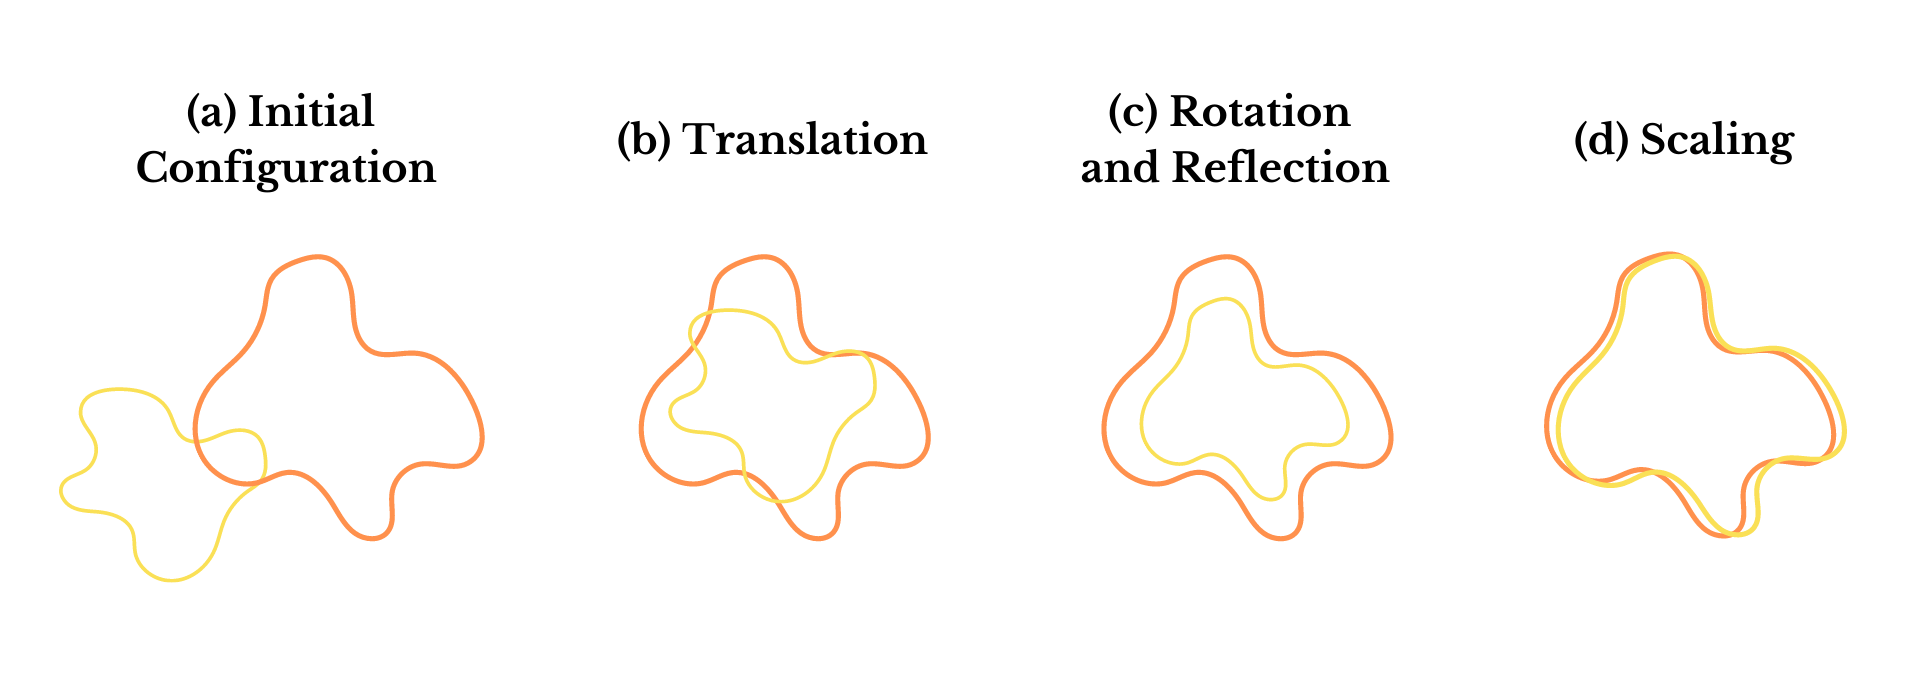
\includegraphics[width=1\linewidth]{sections/figures/orthogonal-procrustes.png}
  \caption{A general of example of the procrustes analysis where translation refers to the geometry transformation of moving every point of a space by the same amount of distance.}
  \label{fig:orthogonal-procrustes}
\end{figure}


On the other hand, the process of alignment is not always necessary for detecting LSC. The use of dynamic word embeddings helps alleviate the need for alignment. Temporal Referencing (TR), presented by \citet{dubossarsky-etal-2019-time}, is a method where diachronic corpora is treated as one corpus—sharing context information across time. This method was motivated by the fact that alignment should be circumvented as \citet{dubossarsky-etal-2017-outta} show that the process introduces noise. TR is a ``relabeling trick to achieve the same goals of the other dynamic methods while using a static embedding method" \citep{tahmasebi-survey2018}. Diachronic corpora are trained synchronically and vectors exist together in one vector space. Word vectors are situated in relation to each other and target words are relabelled and appended with a time-specific token (indicating which corpus they appear in) during training. Relabelling will only occur if the word is a target word. A word \emph{w} will not be relabelled and appear as a ``normal" word vector if it appears as a context word since this information can be shared across time periods. 

\newpage

\section{Experimental Setup}

\subsection{3.1 - Dataset}

The SemEval-2020 Task 1 on Unsupervised Detection of Lexical Semantic Change \citep{schlechtweg-etal-2020-semeval} provides manually-annotated datasets for four languages (English, German, Swedish, and Latin). It is composed of a diachronic corpus pair and a set of target words for each language. Having a gold standard that is based on roughly 100,000 human judgments, researchers now have a more concrete foundation for comparing models. There are two subtasks that differ by the assessment of LSC: binary classification and ranking. In order to identify and evaluate the subtle effects of hyperparameter changes, this thesis follows Subtask 2—based on a ranking of the target words depending on the degree of LSC between the first and second corpus. In contrast to Subtask 1’s binary classification, the method of ranking in Subtask 2 “captures fine-grained changes in the two sense frequency distributions” \citep{schlechtweg-etal-2020-semeval}. The two corpora for each language (C1 and C2) were divided based on data size and the availability of target words. Pre-processing of all corpora involved lemmatization, removal of all punctuation, and randomly shuffling sentences within each time-specific corpora.

The Clean Corpus of Historical American English (CCOHA) consists of different types of text—fiction, non-fiction, magazines, and newspapers—from the 1810s to the 2000s \citep{davies2012expanding, alatrash-etal-2020-ccoha}. The first time-bin corpus used for German is Deutsches Textarchiv (DTA) which is composed of different genres of text from the 16th-20th centuries \citep{dta2017}. For the second time-bin, a combination of the Berliner Zeitung (BZ) and Neues Deutschland (ND) corpora is used \citep{berliner2018,neues2018}. Both German corpora are comprised of newspaper articles from the years of 1945-1993. The corpus used for Latin, LatinISE \citep{mcgillivray-kilgarriff}, is a compilation of texts originating from 2nd century B.C. to 21st century AD from three online digital libraries. The corpora used for Swedish is the Kubhist corpus \citep{Kubhist}, which similar to the German corpus used, is a newspaper corpus with articles from the 18th to the 20th century. \hfill \break
\begin{table}[h]
\small
\centering
\begin{tabular}{l|cc|cc|}
\cline{2-5}
\textbf{}      & \multicolumn{2}{c|}{\textbf{$C_1$}}                    & \multicolumn{2}{c|}{\textbf{$C_2$}}                    \\
                                       & \textit{\textbf{corpus}} & \textit{\textbf{period}} & \textit{\textbf{corpus}} & \textit{\textbf{period}} \\ \hline
\multicolumn{1}{|l|}{\textbf{English}} & CCOHA                    & 1810-1860                & CCOHA                    & 1960-2010                \\ \hline
\multicolumn{1}{|l|}{\textbf{German}}  & DTA                      & 1800-1899                & BZ + ND                  & 1946-1990                \\ \hline
\multicolumn{1}{|l|}{\textbf{Latin}}   & LatinISE                 & -200-0                   & LatinISE                 & 0-2000                   \\ \hline
\multicolumn{1}{|l|}{\textbf{Swedish}} & Kubhist                  & 1790-1830                & Kubhist                  & 1895-1903                \\ \hline
\end{tabular}
\caption{Time periods of each sub-corpora for each language.}
\label{tab:subcorpora-time}
\end{table}
\hfill \break
Annotators—all native speakers or former university students of the respective language they were assigned—were instructed to follow the DURel framework \citep{DURel2018}. Deriving from \citet{blank1997prinzipien}’s continuum of semantic proximity for synchronic polysemy annotation, its semantic-relatedness scale for a target word \emph{w} within two specific time periods from C1 and C2 resulted in high inter-annotator agreement. 
	
Each language is accompanied by a target word list that consists of words that have undergone semantic change or stable words—words that have not changed in meaning. For words that have changed in meaning, it is not distinguished whether words have lost or gained a sense. Stable words were chosen to act as counterparts of words that have changed in meaning through the consideration of the same POS tag and a comparable/similar frequency development between the two time periods. This consideration minimizes possible model biases that result from these factors. \citep{dubossarsky-etal-2017-outta} Since many of the English target words underwent POS-specific semantic changes, POS tags have been concatenated in the target word list (“word\_pos”). Although the addition of POS tags in the SemEval task was for the purpose of English words having a tendency to change POS tags when changing senses, it was also a great opportunity to examine model performances based on POS tags for this project. The addition of POS tags for the target word lists of the remaining three languages will be discussed further below.
 
% Please add the following required packages to your document preamble:
% \usepackage[table,xcdraw]{xcolor}
% If you use beamer only pass "xcolor=table" option, i.e. \documentclass[xcolor=table]{beamer}
\begin{table}[h]
\small
\centering
\begin{tabular}{|c|c|c|c|}
\hline
\textbf{Language} & \textbf{NN} & \textbf{VB} & \textbf{ADJ} \\ \hline
\textit{English}                          & 33          & 4           & 0            \\ \hline
\textit{German}                           & 32          & 14          & 2            \\ \hline
\textit{Latin}                            & 28          & 5           & 7            \\ \hline
\textit{Swedish}                          & 22          & 6           & 3            \\ \hline
\end{tabular}
\caption{Number of nouns (NN), verbs (VB), and adjectives (ADJ) in each language's target word list.}
\label{tab:postag-breakdown}
\end{table}

(FROM MOTIVATION)
\cmtKV[inline]{this section feels out of place but at the same time should be mentioned, just not sure if it's better off in motivation}
Another challenge that the field is currently facing is having a more robust system of evaluation. Currently, semantic annotation stands as the most reliable (sole (TECHNICALLY NOT)) way of evaluating and validating semantic change in historical corpora \citep{hengchen2021challenges}. Although effective (for now), the annotating process to obtain ground-truth data results in large amounts of money and time expended. It also only produces a limited target word list—allowing the possibility of evaluation inconsistencies to be introduced. A model might perform well with one target list and horribly with another. (CONJECTURE? LOL) Using a simulated LSC for evaluation is in its early stages and is encouraged to be used for evaluation in tandem with ground-truth testing.

Numerous types of semantic representations were used by teams during the SemEval task: token embeddings vs. type embeddings and topic modelling vs. vector space models. In both Subtask 1 and 2, the highest-performing systems used static-type embedding models. Token embeddings include more contextual information each time the target word appears in the corpus while type embeddings are average embeddings (LACKING). However, it was pointed out that raw corpora, rather than lemmatized corpora, would bode better for token embeddings. (ANNOTATION?) Following the best-performing models of the tasks, with a larger focus on Subtask 2, a hyperparameter search of models with type embeddings would help determine if the top scores of the task could be surpassed solely on changes in hyperparameters. (ENDSOUNDS WEIRD, EDIT) 

\subsection{3.X - Experimental Large-Scale Hyperparameter Search (TOO LONG?)}
In order to clarify the scope and justify the hyperparameter range for this large-scale hyperparameter search, the results from the SemEval-2020 Task 1 are used as the basis/starting point (PICK ONE). The top-performing models were taken into consideration along with the post-hoc improvements and analyses of those models by \citet{kaiser-etal-2020-ims}. The pipeline was coded and structured with the possibility of reusing the code for conducting similar hyperparameter searches in future LSC tasks with the hopes of the hyperparameter searches to be based on the findings of this thesis—and in turn, hyperparameters with smaller ranges and motivated by linguistic and domain-specific reasoning. 

\cmtKV[inline]{**formatting, also think it would be useful to show the range after each subsubsection heading or would that be redundant, this below could also be neater, need to look into it}
The initial hyperparameters examined and analysed are shown below:
\begin{itemize}
    \item language $\in$ [English, German, Latin, Swedish],
    \item algorithm $\in$ [Word2Vec, FastText],
    \item alignment method $\in$ [Orthogonal Procrustes, Incremental Training],
    \item epochs $\in$ $[5, 10, 20, 50, 100]$,
    \item dimensions $\in$ $[10, 25, 50, 100, 300]$,
    \item frequency threshold $\in$ $[5, 10, 50, 100]$.
\end{itemize}%\vspace{+1ex}


**READABILITY SAKE, not canonically hyperparameters but are included when mentioning combination of hyperparameter

\subsubsection{Algorithm}
Type embeddings were used in the top-performing models for all four languages in Subtask 2.  Since type embeddings overwhelmingly outperformed token embeddings, static-type embeddings were chosen to be implemented. The same is seen in the hyperparameter search conducted by \citet{hengchen2021SBXrushifteval} with Russian data. The skip-gram negative sampling (SGNS) algorithm was used by the top 4 teams whose models performed well in Subtask 2 of the SemEval task. Bidirectional Encoder Representations from Transformers (BERT) was not used as \citet{laicher-2020} demonstrated that it resulted in poor results for an LSC task in Italian. Variety is provided in the algorithm hyperparameter by comparing the use of n-grams of Word2Vec and FastText. Word2Vec has shown success in LSC tasks and the use of FastText would address the morphological considerations for words that should be made as shown by \citet{bojanowski2017enriching}.

\subsubsection{Alignment Method}
The two alignment methods used are Orthogonal Procrustes and incremental training. Orthogonal Procrustes is implemented by using the first time period model as the base and the second time period model is “stretched” to fit the first. This is motivated by the fact that language builds on itself. In order to make comparisons of words changing over time, new usages of already existing words and new words (second time period model) should be made to fit into the contexts and usages that it proceeds (first time period model). The Gensim Word2Vec Procrustes Alignment tutorial by Ryan Heuser\footnote{\url{https://gist.github.com/quadrismegistus/09a93e219a6ffc4f216fb85235535faf}}  was initially used but was not compatible with FastText models. These aligned models were still saved and evaluated. However, all models were then aligned following the implementation of Team UWB @ SemEval \citet{prazak-etal-2020-uwb}’s model implementations using VecMap \footnote{\url{https://github.com/artetxem/vecmap}} by \citet{artetxe2018generalizing}. However, implementation differed from \citet{prazak-etal-2020-uwb}’s since the alignment chosen was supervised due to computational requirements and preliminary tests showed good performance. After seeing the results of VecMap’s supervised alignment method, another hyperparameter was introduced for models that are being aligned through Orthogonal Procrustes. There was an option on how many words can be provided in the training dictionary where the word vectors can be aligned automatically. Given a word \emph{w} from the first time period model, its equivalent to the second time period model would also be w. The additional hyperparameter was the amount of words given to VecMap as equivalents—making aligning the two models “easier” or “more supervised” (WORDING).

Models that have Orthogonal Procrustes as the alignment method will also have this added hyperparameter:
\begin{itemize}
    \item vocabulary size $\in$ $[1000, 5000, 10000, ALL]$
\end{itemize}%\vspace{+1ex}

The second alignment method, incremental training, was implemented by taking the first time period model and continue its training but this time using the second time period corpus. The models being compared will be the model trained on the first time period corpus and the model trained on both the first and second time period corpus.

\subsubsection{Epochs} \label{exp-epochs}
Epochs chosen were initially a very wide range from 5 to 100. A smaller preliminary test for higher epochs were conducted while training Word2Vec to see if there were significant improvements in performance and if it was worth exploring further. It was decided that FastText models trained on 100 epochs should not be pursued further due to computational costs and no added performance. The litmus test was done on Word2Vec models as it will always have less vectors since it operates on a per-word basis rather than FastText which creates vectors based on character \emph{n}-grams. 

\subsubsection{Dimensions}
Variety in dimensions were included in this hyperparameter search due to \citet{kaiser-etal-2020-ims}’s post-hoc analysis of the top-performing models in the SemEval-2020 Task 1 demonstrating that the same models can be outperformed by optimising *vector initialization alignment* (INCLUDE?) dimensionality. Their results also show that frequency-induced noise is introduced through vector space alignment and it is strongly correlated to dimensionality. With higher dimensions, vector representations could learn more specific contexts and usages of the word. However, high vector dimensions may also lead to more noise being introduced in the word representations. 

\subsubsection{Frequency Threshold}
Frequency thresholds can have a significant effect on computational time as well as overall performance. The frequency threshold is the amount of times a word has to appear in a corpus for it to be included in the training of the model. This threshold can either help eliminate words that are not relevant and only introduce noise but it can also eliminate important contexts that could help with the nuanced usages of words, possibly a target word. Exploring this hyperparameter would allow us to see if this hyperparameter has an optimal number when combined with other hyperparameters. 

\subsection{3.X - Evaluation/Spearman's Rank Order Correlation}
For SemEval-2020 Subtask 2 where LSC is quantified as a measurement of change through cosine distances, Spearman’s Rank Order Correlation is calculated as the main statistical measure of overall score. Once the cosine distances are calculated for each target word, they are ranked and compared with the gold truth labels. Spearman's correlation $\rho$ is then calculated along with its p-value. Spearman’s $\rho$ can be any value from -1 to 1 where 1 is a perfect positive correlation between ranks, -1 is a perfect negative correlation between ranks, and 0 is no correlation between ranks. In this task, the best possible score for a model would be 1, meaning that it has ranked the cosine distances exactly like the truth labels. Calculating through ranking rather than direct comparisons (such as the difference between each target word’s cosine distance) was chosen since it allows vector spaces to vary more in size given the large amount of hyperparameter combinations being implemented. (NOT SURE IF THIS IS TRUE OR JUST WORDED BADLY) The same evaluation will be done for each model but with the target words divided by POS-tag. Each model will have a Spearman’s $\rho$ for nouns, verbs, and adjectives. 

\subsection{3.X - Ethical Considerations and Efficiency Adjustments}
\label{exp-ethics}
Initially, 1600 models were planned to be trained for this large-scale hyperparameter search. However, with the deduction of 100-epoch models for FastText and the addition of the vocabulary alignment hyperparameter for the Orthogonal Procrustes alignment method, 4000 models were trained in total. Throughout the training process, it was important to vigilantly take into consideration computational times, storage, and energy usage. As stated above in EPOCHS SECTION, 100-epoch models were trained on Word2Vec first and examined to see if the increase in epochs and therefore computational time and energy used also reflected in the model’s performance. Since it did not show promising results or results that increased in conjunction with time and energy spent, training 100-epoch models for FastText was deemed not worth pursuing further. 

The longer period of planning the pipeline was to ensure that once training begins, there are as little road blocks as possible. This would ensure that the training process and the storing of models were always organised and never lost or having to be retrained to avoid unnecessary consumption of resources. In hopes of remaining vigilant and conscious of the large amount of energy, resources, and storage being used for this thesis, adjustments to help with time and energy consumption were constantly being made to the pipeline. After the large-scale pipeline and the Orthogonal Procrustes alignment was incompatible with FastText models, the pipeline was restructured and already existing models were reformatted for efficiency purposes. Before the reformatting, 1TB of data and models were being stored. They were then transferred and reformatted as text files. To save computational time and energy, the cosine distances for the target words of each model were stored as text files and will be made available to the public along with the model text files and pipeline. This was incredibly helpful since the initial plan was for the model to iterate through the entire model to search for the target words and calculate the overall Spearman’s $\rho$ and again for nouns, verbs, and adjectives. Another adjustment made during training was for the incremental alignment method. The model trained on the first time period corpus with the same hyperparameter combinations but for the Orthogonal Procrustes alignment method was used and trained again with the second time period corpus. This eliminated training what would have been 720 duplicate models.  

This large undertaking was done using an Intel Xeon CPU E5-2640 v4 (25M Cache, 2.40 GHz). With about X hours total of training and computational time, around XX kg of CO\textsubscript{2} has been used which equates to X bananas, or X kilometers driven, or X avocados from Mexico.\footnote{\url{https://www.weforum.org/agenda/2020/02/avocado-environment-cost-food-mexico/}} These calculations were made through the CO\textsubscript{2} GU mltgpu tutorial\footnote{\url{https://github.com/faustusdotbe/CO2_GU_mltgpu/blob/main/mltgpu_co2.ipynb}} by Simon Hengchen. These statistics are incredibly important to disclose considering the vast environmental impact conducting these experiments will have. 
\citet{strubell-etal-2019-energy} states that the most computationally-hungry models typically obtain the highest scores. \citet{strubell-etal-2019-energy} also raises awareness on the CO\textsubscript{2} consumption within the NLP community and the importance of reporting of train times and sensitivity to hyperparameters. By providing these statistics, the overall scores, and other files that require computational time and energy consumption, others are able to  further explore and examine this task without having to do all of the model training again. The reporting and analysing of hyperparameter sensitivities and patterns between the models will also allow researchers to apply the intuition when selecting hyperparameters in order to train models that are efficient, environmentally conscious, and yield the best results.



\newpage

\section{Results and Discussion}
\label{sec:results}

\subsection{Overall Top Models}

Hyperparameter searches are purely experimental and can be infinitely expanded. By using the most often used hyperparameter values in LSC tasks, a foundation is made for where to begin. \autoref{fig:score-dist} shows the distribution of Spearman's $\rho$ scores for English, German, Latin, and Swedish respectively. The wide variations of scores for each language in these distributions demonstrate the lack of understanding in the effects of the interactions between hyperparameters on the overall performance of the models. Latin's score distribution in \autoref{fig:score-dist-lat} indicates that most of the models trained resulted in an average score. Without a hyperparameter search, there is a high chance that the model trained on Latin corpora will have an average score hence a much smaller chance of having a model that performs very well. Contrastively, the score distributions for English, German, and Swedish in  \autoref{fig:score-dist-eng}, \autoref{fig:score-dist-deu}, and \autoref{fig:score-dist-sve} respectively, have a much wider range of scores⁠⁠—indicating that hyperparameter searches are also worth conducting. Majority of the 3 figures' model scores are low or average and the top-performing models only make up a small percentage of the total scores. These three languages have a better chance of getting a better-performing model, but also have a higher risk of getting a model that performs very poorly. More evident in \autoref{fig:score-dist-sve}, Swedish is at a higher risk of having a model that will perform poorly due do its incredibly large range of scores. A general analysis of the overall top-performing models for each language will be analysed in this section. Findings of the effects of each hyperparameter on the performance for each language will also be discussed below. 

\begin{figure}[h]
  \centering
  \subcaptionbox{\label{fig:score-dist-eng}English}{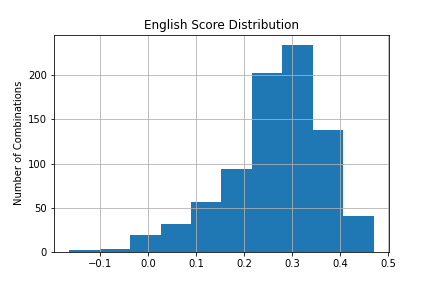
\includegraphics[width = 3in]{sections/figures/eng_score_distribution.png}}\quad
  \subcaptionbox{\label{fig:score-dist-deu}German}{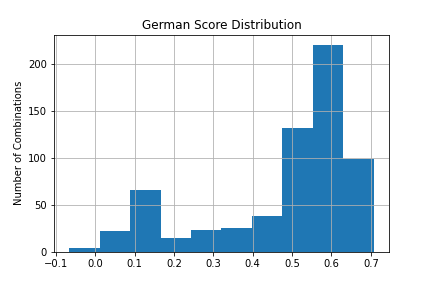
\includegraphics[width = 3in]{sections/figures/deu_score_distribution.png}}\\
  \subcaptionbox{\label{fig:score-dist-lat}Latin}{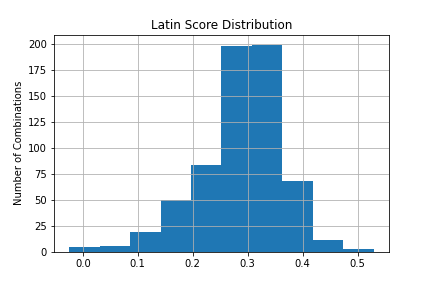
\includegraphics[width = 3in]{sections/figures/lat_score_distribution.png}}\quad
  \subcaptionbox{\label{fig:score-dist-sve}Swedish}{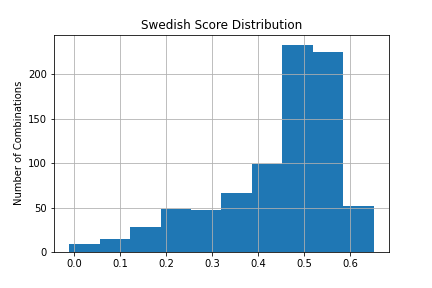
\includegraphics[width = 3in]{sections/figures/sve_score_distribution.png}}
  \caption{Distribution of Spearman's $\rho$ scores for each language.}
  \label{fig:score-dist}
\end{figure}


The hyperparameter search successfully found model combinations that outperformed both the best teams in the SemEval task and \citet{kaiser-etal-2020-ims}’s post-hoc optimizations for both English and Latin. As seen in \autoref{tab:performance-comparison}, a model was found to surpass the score of the best team in SemEval but not \citet{kaiser-etal-2020-ims} for the German language. The top-performing models for each language and their hyperparameters are shown in \autoref{tab:top-models}. Although it is important to analyse the top results for each language separately, it is noteworthy to see commonalities between all four languages. The Orthogonal Procrustes alignment method seems to be the most effective for bigger datasets. For smaller datasets such as Latin, the Incremental Training alignment method is the most effective as the second time period model has information learned from both the first and second time period corpora. Epochs were also surprisingly low and lower frequency thresholds performed best as it included the maximum amount of words in the model’s vocabulary. Typically, longer epochs mean more time for the model to learn more from the data and the nuances within that data. However, there is a certain threshold where the model stops learning what is useful and begins to learn noise which can decrease model performance. 


\begin{table}[h]
\centering
\begin{tabular}{lccc} 
\toprule
\textbf{ } & \textbf{SemEval } & \textbf{\citet{kaiser-etal-2020-ims} }         & \textbf{Best }            \\
English    & \textit{ .422 }   & \textit{ .460 }          & \textbf{\textit{ .469 }}  \\
German     & \textit{ .725 }   & \textit{\textbf{ .780 }} & \textit{ .706 }           \\
Latin      & \textit{ .462 }   & \textit{ .410 }          & \textbf{\textit{ .529 }}  \\
Swedish    & \textit{ .604 }   & \textit{\textbf{ .670 }} & \textit{ .651 }           \\
\bottomrule
\end{tabular}
\caption{Top $\rho$ score comparison between SemEval-2020 Task 1 Subtask 2 teams, \citet{kaiser-etal-2020-ims}, and results.}
\label{tab:performance-comparison}
\end{table}


\begin{table}[h]
\centering
\begin{tabular}{cccccccc} 
\toprule
\textbf{ } & \textbf{ Algorithm } & \textbf{ Alignment } & \textbf{ Vocab Size } & \textbf{ Epochs } & \textbf{ Dims } & \textbf{ Freq Threshold } & \textbf{ $\rho$ }  \\
English    & FT              & OP               & ALL (16429)      & 5                 & 300             & 10               & .469            \\
German     & W2V             & OP               & ALL (218507)     & 5                 & 25              & 5                & .706            \\
Latin      & W2V             & INC              & -                & 5                 & 10              & 10               & .529            \\
Swedish    & FT              & OP               & 5000             & 10                & 50              & 10               & .651            \\
\bottomrule
\end{tabular}
\caption{Top-performing models for each language and their parameters. Abbreviations: W2V=Word2Vec, FT=FastText, OP=Orthogonal Procrustes, INC=Incremental.}
\label{tab:top-models}
\end{table}

The following analyses will show the differences in scores when the top-performing model is taken for each language and each hyperparameter is kept the same except for one hyperparameter. For example, Latin’s best model has the hyperparameters: Word2Vec, Incremental Training, 5 epochs, 10 dimensions, 10 frequency threshold. To explore the effects of the change in epochs, all the hyperparameters will remain the same except for epochs. The scores for each of these models are represented by a point in the graph where the $x$-axis is the hyperparameter in question and the $y$-axis is the Spearman's $\rho$ score. These points are joined by a dotted line graph and each line represents one of the four languages. Points that are in grey are statistically insignificant where p-value > 0.05 but they are included for informational purposes. Individual hyperparameter graphs for each language are available in \autoref{app-topmodelgraphs}. In order to extrapolate information from the data collected, the dotted lines are created in order to see trends between the points. However, it is acknowledged that if models were actually trained for each increase in the hyperparameter in question, there is a possibility that the trends may differ. 
%\cmtKV[inline]{should i write the last sentence to sound less invalidating (alternative phrase "trends in reality could show very different results."}

The relationship between epochs and performance raises the question of priority of performance and environmental impact. In \autoref{fig:all-epochs}, English and Swedish do not have 100-epoch models since it was deemed that their improved performance return was minimal compared to the time spent and energy consumed for training (discussed further in Section~\ref{exp-epochs}). There is a general decline in $\rho$ as epochs are increased for English, Latin, and Swedish while German had a slight increase in $\rho$ from 50 to 100 epochs. German and Latin appear to experience a similar decrease by 20 epochs but diverge after 50 epochs where German increases and Latin significantly decreases. As seen in \autoref{tab:subcorpora-size}, the German diachronic corpora has a total of 142.5 million tokens while the Latin diachronic corpora has 11.1 million tokens. This divergence might be attributed to the dataset size since the German corpora is much larger and there is more for the model to learn as epochs are increased.  On the other hand, the Latin corpora is very limited and after 50 epochs, the decrease in $\rho$ could be additional noise being introduced to the model. Although there might still be an increase in performance when training for more than 50 or 100 epochs, lower epochs seem to be the better choice for LSC. It also is a question of priority—smaller epochs or spending more time, memory, and energy. For this hyperparameter, the option to have a smaller environmental impact and economic cost compromises very little in terms of performance compared to the performance differences between lower epochs. Economic (both money and time) as well as environmental costs of longer training times for a slightly higher accuracy score is something that must be considered given the ongoing impacts of climate change on our planet. This consideration will be discussed further in Section~\ref{sec:ethicalcons}.

%\cmtKV[inline]{phrasing of last part}

%\cmtKV{is the last sentence more opinionated, should it be included, how could i word it to not sound as opinionated}

\begin{figure}[h]
  \centering
  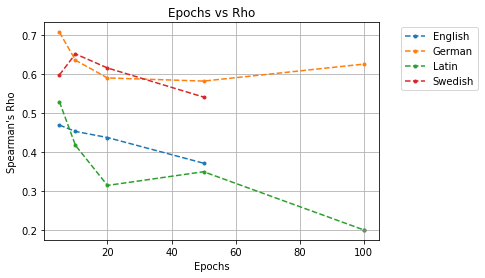
\includegraphics[width=.8\linewidth]{sections/figures/epochs_all.png}
  \caption{Change in Epochs vs. Performance.}
  \label{fig:all-epochs}
\end{figure}

The vector dimension hyperparameter refers to the size of the vector for each word representation. Increasing vector dimensions requires a higher computational time and more memory. As expected, English performs best with higher dimensions. The 300-dimension hyperparameter is common in NLP tasks and is usually the standard when conducting NLP (including LSC) tasks on other languages due to the prevalence in studies being done in English.\footnote{Using vectors with a size of 300 dimensions for word representations is the agreed upon standard and is used in most work and tutorials in NLP.} As seen in \autoref{fig:all-dims}, choosing higher dimensions does not necessarily result in better $\rho$ scores as it does with the English language. German, Swedish, and Latin all have higher $\rho$ scores when lower dimensions are used. Latin’s top model performed best with the lowest dimension of 10. Since the Latin corpora is very small compared to the other three languages, having less abstractions of words in the vector representations might have been more useful for the model and minimised the introduction of noise. The genre makeup of corpora is also put into question as it seems to have an effect on the vector dimensions consequently affecting performance. Swedish and German are both composed of newspaper corpora and so the same style and type of language is used. English has a mixed genre corpora and Latin is somewhere in between. Since Swedish and German models are trained on texts that have their own writing style where constructions of sentences are similar but the words have been used under many contexts, vectors with higher dimensions allow for those nuances to be learned. On the other hand, the Latin corpora consists of a wide range of texts compiled and vectors with lower dimensions allow the model to learn the usages of the words in a broader context. The genres of text being included in the corpora must be taken into consideration before choosing the vector dimensions for a model. The standard convention of 300 dimensions, based on English results in past NLP tasks, also shows not as effective on other languages.

%\cmtKV{should i cite something here or is this okay to just say}

\begin{figure}[h]
  \centering
  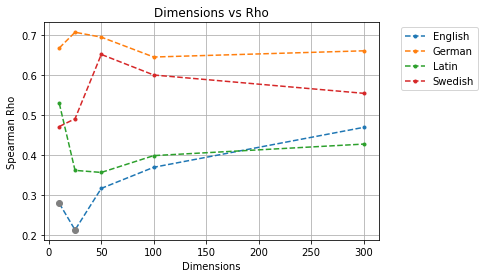
\includegraphics[width=.8\linewidth]{sections/figures/dims_all.png}
  \caption{Change in Dimensions vs. Performance.}
  \label{fig:all-dims}
\end{figure}

The frequency threshold hyperparameter refers to the minimum number of times a word has to appear in a corpus to be included in the model’s vocabulary and thus for a vector to be learned. Smaller frequency thresholds will result in a larger vocabulary. Since the vocabulary is larger, memory needed will also be larger as there are more vectors to be stored and learned by the model.  \autoref{fig:all-freqs} illustrates that it is generally better to have a lower frequency threshold in order to ensure that majority of the words in a corpus is being included. German and Swedish do not have 4 points in \autoref{fig:all-freqs} as the $\rho$ scores for those model combinations were NaNs. While German performs best with the lowest frequency threshold of 5, English, Latin, and Swedish all perform better at a slightly higher frequency threshold of 10. Depending on the corpus being used, better performance with a higher frequency threshold could mean an effective filtering out of words that are seldom used in the corpus and do not effectively contribute to the target words' contextual meanings: a steady decrease in $\rho$ scores are seen as the frequency threshold increases. This is expected since a higher frequency threshold results in less words in the vocabulary and a smaller vocabulary naturally excludes words that contribute to the contextual meaning of a word. 

\begin{figure}[h]
  \centering
  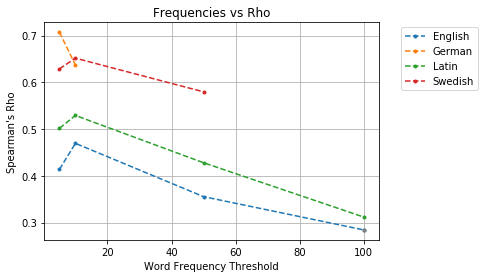
\includegraphics[width=.8\linewidth]{sections/figures/freqs_all.png}
  \caption{Change in Frequency Thresholds vs. Performance.}
  \label{fig:all-freqs}
\end{figure}

Two approaches were used for the Orthogonal Procrustes alignment method—Ryan Heuser’s Tutorial\footnote{\url{https://gist.github.com/quadrismegistus/09a93e219a6ffc4f216fb85235535faf}} and VecMap\footnote{\url{https://github.com/artetxem/vecmap}}. The former had a default of including the entire shared vocabulary of the first time period corpus and the second time period corpus during the alignment process. However, the latter included the option to indicate the size of the shared vocabulary during the alignment process. \autoref{fig:all-vocabalign} shows the effect of vocabulary size during the Orthogonal Procrustes alignment process on $\rho$ scores when using VecMap. Latin is not included in this graph since its top-performing model used the Incremental Training alignment method. English and German seem to be affected similarly from this hyperparameter while Swedish experiences the opposite. German profits when the entire vocabulary (where the shared vocabulary size is 218,507), including the target words, is included in the alignment process and results in the top-performing model. Swedish experiences a similar increase in performance when the shared vocabulary size is 5000. However, the top-performing model for Swedish has a vocabulary size of 5000 and an increase in vocabulary size shows a decrease in $\rho$ scores. Although English has a significantly smaller corpora size, it also profits from the inclusion of the entire vocabulary (where the shared vocabulary size is 16,429) when aligning both time period models. \autoref{fig:all-vocabalign} shows that the most effective shared vocabulary size when using the Orthogonal Procrustes alignment method is language-specific and cannot be generalised. It also demonstrates the advantages of performing hyperparameter searches and that findings in one language are not always universal.

\begin{figure}[h]
  \centering
  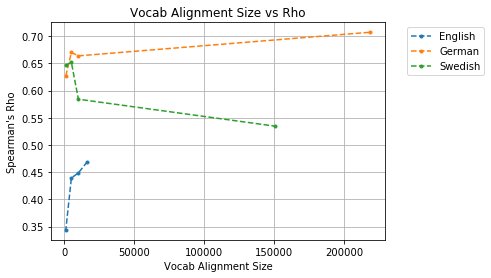
\includegraphics[width=.8\linewidth]{sections/figures/vocabalignment_all.png}
  \caption{Shared Vocabulary Size in Orthogonal Procrustes Alignment vs. Performance.}
  \label{fig:all-vocabalign}
\end{figure}

The results from this large-scale hyperparameter search introduces and substantiates some intuitions when selecting hyperparameters for future LSC tasks. There is a threshold for the amount of improvement in scores when models are trained with higher epochs. Models trained with generally lower epochs performed the best within the range chosen for this hyperparameter search. The standard of 300 dimensions as a baseline for vector representations, based on NLP best prractices for the English language, does not necessarily apply to all languages. German, Latin, and Swedish performed best with models that had lower dimensions. When choosing the dimensions of vectors, it is also important to consider the size of the corpora and the genres of texts included in the corpora. Larger corpora where the usage of words fall under the same writing style might need higher dimensions in order to learn the nuances whenever a word is used. Conversely, corpora smaller in size consisting of texts of a wider genre range would need lower dimensions in order to learn the usages of words in a broader context. In terms of frequency thresholds, a lower frequency threshold maximises the amount of words included in the vocabulary and this results in more contributions to the contextual meaning of each word. However, a slightly higher frequency threshold can be effective in filtering out words that are rarely used and do not contribute to the meaning of the target words. For models that perform better using the Orthogonal Procrustes alignment method, the size of the shared vocabulary during the aligning process can greatly affect the performance. Both English and German profit from including the entire shared vocabulary while Swedish performs better with a smaller shared vocabulary.

\subsection{Top Models Based on POS-Tag}

Every model trained was also evaluated by creating smaller target word lists based on each target word’s POS-tag. For each language’s target word list, the words have been manually annotated\footnote{Thank you to Dr. Barbara McGillivray, Konstantinos Mavromatakis, Merle Pfau, and Saga Hansson for manually annotating the Latin, German, and Swedish target word lists.} and POS-tagged as either a noun (nn), verb (vb), or adjective (adj). The target word list breakdown for each language is seen in \autoref{fig:target-postags}. Nouns are much more prevalent in the target word lists and so conclusions made for nouns are better grounded compared to conclusions made for verbs and adjectives. Control words within each POS-tag are indicated through a lighter colour respective of its POS-tag and offsetted in \autoref{fig:target-postags}. With already a smaller ratio and an addition of control words that have a 0 change score, a $\rho$ score of 1 can sometimes be more easily attained since it is calculated by rank. For example, \autoref{fig:postag-deu} shows that there are only 2 German target words that are adjectives and one is a control word. A model’s chances of obtaining a perfect Spearman's $\rho$ score of 1 is very high since the control word's change score would be zero—making it very likely to have the correct ranking. 

%\cmtSH[inline]{Could you perhaps try to stick "the block of the same colour" together in the figure? Eg in Swedish and German. It's currently also difficult to know eg if the values for "nn" include those for "nn-control"}
%\cmtKV[inline]{REARRANGE PIE SLICES}
%\cmtSH{It would be wiser to rename, in the plot itself, "nn" to "nn-change" -- otherwise it's unclear whether nn-control is part of nn without doing the addition} 

\begin{figure}[h]
  \centering
  \vspace*{-2mm}
  \subcaptionbox{\label{fig:postag-eng}English (89$\%$ nouns, 11$\%$ verbs)}{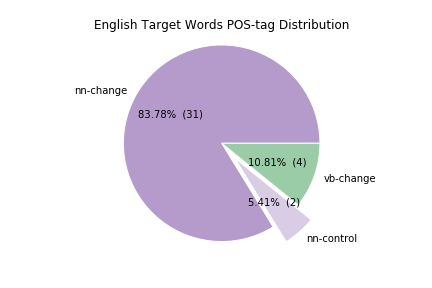
\includegraphics[width = 3in]{sections/figures/eng-pos-target-control.png}}\quad
  \subcaptionbox{\label{fig:postag-deu}German(67$\%$ nouns, 29$\%$  verbs, 4$\%$ adjectives)}{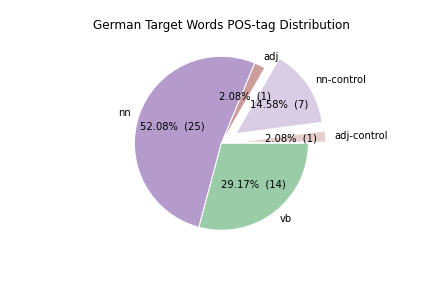
\includegraphics[width = 3in]{sections/figures/deu-pos-target-control.png}}\\
  \subcaptionbox{\label{fig:postag-lat}Latin (70$\%$ nouns, 12.5$\%$  verbs, 17.5$\%$ adjectives)}{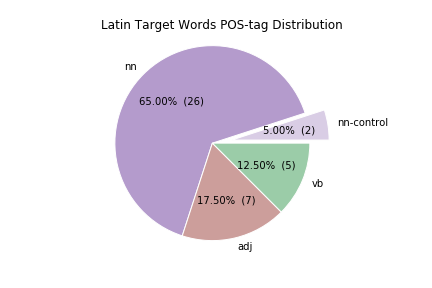
\includegraphics[width = 3in]{sections/figures/lat-pos-target-control.png}}\quad
  \subcaptionbox{\label{fig:postag-sve}Swedish (71$\%$ nouns, 19$\%$ verbs, 10$\%$ adjectives)}{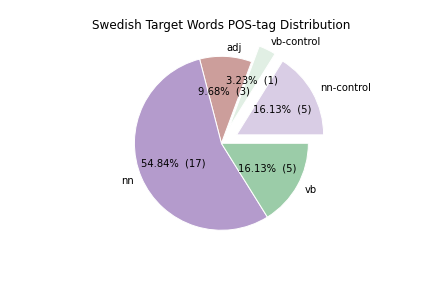
\includegraphics[width = 3in]{sections/figures/sve-pos-target-control.png}}
  \caption{Target Word POS-tag Distribution for Each Language. Control words (words that have not undergone semantic change) are shown through a lighter colour respective of its POS-tag and offsetted. Percentages in the captions are rounded to the nearest integer for readability.}
  \label{fig:target-postags}
\end{figure}

The tables below (\autoref{tab:eng-posresults}, \autoref{tab:deu-posresults}, \autoref{tab:lat-posresults}, \autoref{tab:sve-posresults}) for each language show the top-performing models based on the smaller target word lists created by sorting the target words by POS-tag. For each table, the first row is the overall top-performing model (entire target word list), included for easier comparisons to models that performed well detecting LSC for specific POS-tags. A $\Delta$ column is also included which shows the difference in performance between the overall top-performing model and the POS-tag specific models that had the highest scores. 

In the per POS-tag evaluation of models for English seen in \autoref{tab:eng-posresults}, it was interesting to see that every top-performing model, including the overall top-performing model, had the dimensions hyperparameter at 300. For all the POS-tag evaluations, higher epochs seem to have helped with increasing the $\rho$ score. However, it is important to keep in mind that there are only 4 verbs out of the 33 English target words. Since nouns makeup over 87\% of the English target word list, it makes sense that the top-performing model for nouns has a very similar hyperparameter combination as well as $\rho$ score. There is no top-performing model for adjectives since the English target word list did not have any adjectives. 


Word2Vec is prevalent in the German per POS-tag evaluation of models. As seen in \autoref{tab:deu-posresults}, there were 670 hyperparameter combinations that all obtained the perfect $\rho$ score of 1. There are only 2 adjectives out of 48 German target words and 1 adjective was a control word (where its change score was 0). With this in mind, there is a higher chance that models would obtain a $\rho$ score of 1 since it is calculated through ranking. On the other hand, verbs makeup 29\% of the target words and the top-performing model scored quite well with only a $\Delta$ of 0.096. Overall, smaller dimensions result in better scores for the German target word list. 


The POS-tag evaluation of models for Latin seen in \autoref{tab:lat-posresults} had the greatest differences in hyperparameters compared to its overall top-performing model. All of the top-performing models for each POS-tag also had higher $\rho$ scores. All of the top-performing models for adjectives had Orthogonal Procrustes as the alignment method and surprisingly much higher epochs, dimensions, and frequencies—most being 50 epochs, 25 dimensions, and 100 frequency threshold. The high frequency threshold might be due to the high frequency of adjectives within the corpora. Majority of the words would have been then filtered out leaving a higher chance of very few words being left including the adjectives. The top-performing model for nouns had a higher $\rho$ score by a $\Delta$ of 0.174 but shares the same hyperparameters as the overall top-performing model except for the algorithm (FastText instead of Word2Vec) and a higher frequency threshold. Top-performing models for verbs (making up 12.5\% of the target words) tend to get better results with lower frequency thresholds.


Top-performing models for Swedish based on target word POS-tags seen in \autoref{tab:sve-posresults} were a bit scattered but still had commonalities. The most common for all POS-tag evaluations were 50 epochs, 100 dimensions, and 10 frequency threshold. Only the top-performing model for adjectives performed better than the overall top-performing model scoring a $\rho$ of 1 by a $\Delta$ of 0.349. However, there are only 3 adjectives out of the 31 Swedish target words. All of the top-performing models for verbs and nouns along with one of the top-performing models for adjectives have Incremental Training as the alignment method (contrasting the overall top-performing which has Orthogonal Procrustes) indicating that Incremental Training must learn something specific when it comes to detecting LSC for Swedish POS-tags. 

% bad conduct
%\bigskip
%\bigskip

\begin{table}[h]
\centering
\begin{tabular}{cccccccccc} 
\toprule
\textbf{ Algo } & \textbf{ Align } & \textbf{ Vocab Size } & \textbf{ Epochs } & \textbf{ Dims } & \textbf{ Freq} & \textbf{ Lg } & \textbf{ POS } & \textbf{ Rho } & \textbf{ $\Delta$ }  \\
FT              & OP               & ALL (16429)           & 5                 & 300             & 10             & ENG           & -              & .469           & -               \\
-               & -                & -                     & -                 & -               & -              & ENG           & ADJ            & -              & -               \\
FT              & INC              & -                     & 10                & 300             & 10             & ENG           & NN             & .463           & -0.005            \\
FT              & INC              & -                     & 50                & 300             & 5              & ENG           & VB             & .800           & +0.331            \\
FT              & INC              & -                     & 50                & 300             & 50             & ENG           & VB             & .800           & +0.331            \\
W2V             & OP               & -                     & 50                & 300             & 100            & ENG           & VB             & .800           & +0.331            \\
W2V             & OP               & 1000                  & 20                & 300             & 10             & ENG           & VB             & .800           & +0.331            \\
W2V             & OP               & 1000                  & 50                & 300             & 100            & ENG           & VB             & .800           & +0.331            \\
W2V             & OP               & 10000                 & 20                & 300             & 10             & ENG           & VB             & .800           & +0.331            \\
\bottomrule
\end{tabular}
\caption{English Top-performing Models for Each POS-tag. Abbreviations: W2V=Word2Vec, FT=FastText, OP=Orthogonal Procrustes, INC=Incremental, ADJ=Adjectives, NN=Nouns, VB=Verbs.}
\label{tab:eng-posresults}
\end{table}


%** WHERE IS THE MISSING DOLLAR SIGN\cmtSH{This was $^*$  for MODELS, fixed now -- the circonflex needs math mode to mean "to the x power"}
\begin{table}[h]
\centering
\begin{tabular}{cccccccccc} 
\toprule
\textbf{ Algo } & \textbf{ Align } & \textbf{ Vocab Size } & \textbf{ Epochs } & \textbf{ Dims } & \textbf{ Freq } & \textbf{ Lg } & \textbf{ POS } & \textbf{ Rho } & \textbf{ $\Delta$ }  \\
W2V             & OP               & ALL (218507)          & 5                 & 25              & 5              & DEU           & -              & .706           & -               \\
670             & MODELS$^*$       & GOT                   & SAME              & SCORE           & FOR            & DEU           & ADJ            & 1.00           & +0.294          \\
W2V             & INC              & -                     & 20                & 10              & 10             & DEU           & NN             & .187 (p=0.30)  & -0.518          \\
W2V             & INC              & -                     & 5                 & 50              & 5              & DEU           & VB             & .609           & -0.096          \\
\bottomrule
\end{tabular}
\caption{German Top-performing Models for Each POS-tag. $^*$670 models had a Spearman's $\rho$ score of 1 since there were only 2 adjectives in the German target word list where one was a control word (zero change). Please refer to the POS-tag results file available in \autoref{app-resources}. Abbreviations: W2V=Word2Vec, FT=FastText, OP=Orthogonal Procrustes, INC=Incremental, ADJ=Adjectives, NN=Nouns, VB=Verbs.}
\label{tab:deu-posresults}
\end{table}


\begin{table}[h]
\centering
\begin{tabular}{cccccccccc} 
\toprule
\textbf{ Algo } & \textbf{ Align } & \textbf{ Vocab Size } & \textbf{ Epochs } & \textbf{ Dims } & \textbf{ Freq } & \textbf{ Lg } & \textbf{ POS } & \textbf{ Rho } & \textbf{ $\Delta$ }  \\
W2V             & INC              & -                     & 5                 & 10              & 10             & LAT           & -              & .529           & -               \\
W2V             & OP               & 1000                  & 50                & 25              & 100            & LAT           & ADJ            & .821           & +0.291          \\
FT              & OP               & 5000                  & 50                & 25              & 100            & LAT           & ADJ            & .821           & +0.291          \\
FT              & OP               & 10000                 & 50                & 25              & 100            & LAT           & ADJ            & .821           & +0.291          \\
FT              & OP               & ALL (1911)            & 50                & 25              & 100            & LAT           & ADJ            & .821           & +0.291          \\
FT              & INC              & -                     & 10                & 10              & 100            & LAT           & ADJ            & .821           & +0.291          \\
FT              & INC              & -                     & 20                & 25              & 100            & LAT           & ADJ            & .821           & +0.291          \\
FT              & INC              & -                     & 5                 & 10              & 50             & LAT           & NN             & .704           & +0.174          \\
W2V             & INC              & -                     & 5                 & 25              & 10             & LAT           & VB             & 1.0            & +0.471          \\
W2V             & INC              & -                     & 5                 & 100             & 10             & LAT           & VB             & 1.0            & +0.471          \\
W2V             & INC              & -                     & 5                 & 300             & 5              & LAT           & VB             & 1.0            & +0.471          \\
W2V             & INC              & -                     & 5                 & 300             & 10             & LAT           & VB             & 1.0            & +0.471          \\
W2V             & INC              & -                     & 10                & 100             & 5              & LAT           & VB             & 1.0            & +0.471          \\
W2V             & INC              & -                     & 10                & 300             & 10             & LAT           & VB             & 1.0            & +0.471          \\
W2V             & INC              & -                     & 20                & 300             & 10             & LAT           & VB             & 1.0            & +0.471          \\
W2V             & INC              & -                     & 50                & 300             & 10             & LAT           & VB             & 1.0            & +0.471          \\
W2V             & INC              & -                     & 100               & 300             & 10             & LAT           & VB             & 1.0            & +0.471          \\
FT              & INC              & -                     & 20                & 100             & 10             & LAT           & VB             & 1.0            & +0.471          \\
FT              & INC              & -                     & 20                & 300             & 5              & LAT           & VB             & 1.0            & +0.471          \\
FT              & INC              & -                     & 50                & 100             & 5              & LAT           & VB             & 1.0            & +0.471          \\
\bottomrule
\end{tabular}
\caption{Latin Top-performing Models for Each POS-tag. Abbreviations: W2V=Word2Vec, FT=FastText, OP=Orthogonal Procrustes, INC=Incremental, ADJ=Adjectives, NN=Nouns, VB=Verbs.}
\label{tab:lat-posresults}
\end{table}


\begin{table}[h]
\centering
\begin{tabular}{cccccccccc} 
\toprule
\textbf{ Algo } & \textbf{ Align } & \textbf{ Vocab Size } & \textbf{ Epochs } & \textbf{ Dims } & \textbf{ Freq } & \textbf{ Lg } & \textbf{ POS } & \textbf{ Rho } & \textbf{ $\Delta$ }  \\
FT              & OP               & 5000                  & 10                & 50              & 10                        & SVE           & -              & .651           & -               \\
FT              & OP               & 1000                  & 50                & 100             & 50                        & SVE           & ADJ            & 1.0            & +0.349          \\
FT              & INC              & -                     & 50                & 300             & 50                        & SVE           & ADJ            & 1.0            & +0.349          \\
W2V             & OP               & 1000                  & 50                & 100             & 50                        & SVE           & ADJ            & 1.0            & +0.349          \\
W2V             & OP               & 5000                  & 20                & 300             & 10                        & SVE           & ADJ            & 1.0            & +0.349          \\
W2V             & OP               & -                     & 10                & 100             & 10                        & SVE           & ADJ            & 1.0            & +0.349          \\
W2V             & INC              & -                     & 20                & 10              & 10                        & SVE           & NN             & .464           & -0.187          \\
FT              & INC              & -                     & 50                & 100             & 100                       & SVE           & VB             & .371           & -0.280          \\
W2V             & INC              & -                     & 20                & 10              & 10                        & SVE           & VB             & .371           & -0.280          \\
W2V             & INC              & -                     & 50                & 10              & 5                         & SVE           & VB             & .371           & -0.280          \\
\bottomrule
\end{tabular}
\caption{Swedish Top-performing Models for Each POS-tag. Abbreviations: W2V=Word2Vec, FT=FastText, OP=Orthogonal Procrustes, INC=Incremental, ADJ=Adjectives, NN=Nouns, VB=Verbs.}
\label{tab:sve-posresults}
\end{table}

% this is probably bad conduct
%\bigskip
%\bigskip
%\bigskip
%\bigskip
POS-tag evaluation of all the models trained shows that there are hyperparameter combinations that perform better when detecting LSC for specific POS-tags than the overall top-performing model. It also shows that some hyperparameter combinations can be used in order to better detect LSC depending on the target words’ POS-tag. 


\newpage

\section{Ethical Considerations}
\label{sec:ethicalcons}

Ethical considerations must be made when conducting an experimental research method, as with a hyperparameter search. The effects of conducting this experiment is critically assessed and evaluated through environmental and sociological lenses.

Throughout the process of the hyperparameter search, environmental impact was considered at each step. While adjustments were made to minimise environmental impact, they also help create a more efficient and robust pipeline. As discussed in Section~\ref{exp-ethics}, the project had a total of approximately 430 hours of training and computational time spent and 1.372 kg of CO\textsubscript{2} consumed. For Word2Vec models, the shortest training time was less than 1 second\footnote{Many models had this same training time. An example model trained on the English corpora had the hyperparameters: Alignment=Orthogonal Procrustes, Epochs=5, Dimensions=10, Frequency Threshold=5.} and the longest was around 3 hours and 26 minutes\footnote{This model trained on the Swedish corpora had the hyperparameters: Alignment=Orthogonal Procrustes, Epochs=100, Dimensions=25, Frequency Threshold=100.}. After training all of the model combinations that use the Word2Vec algorithm, results were evaluated and it was decided that training 160 model combinations that required 100 epochs each of training for FastText would not produce significant or meaningful results. Since FastText aims to create character \emph{n}-gram vector representations, training 100-epoch models would involve much more computational time and memory usage compared to the already large models that were created using Word2Vec. Despite acknowledgments and modifications for minimising consumption and efficiency reasons, a significant amount of energy and memory being used is inevitable during a large-scale hyperparameter search. To ensure that the energy consumed and the space taken is worthwhile, all of the results and pipeline will be available for public access (see \autoref{app-resources}). The POS-tagged word lists and cosine distances for each model will also be available for further analysis and future evaluations. This large-scale hyperparameter search is also well-documented to ensure that it will not have to be done again and future tasks can focus on refining model optimisations. 

Another crucial consideration that must be made is regarding the data and the type of content being used for training models. Humans have written the texts in these corpora and humans are inherently biased. Anonymity is also a concern for researchers when using text as data. Most of the historical texts used for this thesis are quite old, spanning from 2\textsuperscript{nd} century B.C. to 2010 with most of the texts coming from the 1800s-1900s. Given the age of the texts being used, the question of anonymity and privacy is not a large concern for this thesis. Through training, machines inevitably learn the biases from these past texts. Biases such as racism, sexism, homophobia, and other forms of discrimination towards marginalised groups of people can be seen throughout historical texts. \citet{tripodi-etal-2019-tracing} show that antisemitic language can be detected through language change. It is vital to acknowledge that these inherent biases exist within historical texts. Despite releasing these models, which have learned and reinforced these biases, I do not endorse, nor agree with these biases. As \citet{hengchen-tahmasebi_2021-swedishdiachronic} state, the hope is to “shed light on these representations, as ignoring them would mean they have never existed”. 


\newpage

\section{Critiques and Limitations}
\label{sec:critiques}

The common and most effective approach in detecting language change still presents limitations and makes many assumptions that must be acknowledged and discussed. This section will discuss components of semantic change that are overlooked with the approach used for this thesis and its shortcomings. 

As with any task, different approaches have different aims and results. When detecting LSC through vector representations, the choice of what each vector represents can significantly change the results. For this thesis, each word in the vocabulary is represented by one vector only. However, by doing so the meaning of a word is limited, or arguably broadened. Words that have more than one sense or meaning will only be represented by an average of all of the times the word has been used in the corpus. This word vector representation can then be affected by the frequencies of the senses. If one sense appears more in a corpus than the other, its representation will skew towards the sense that is more prevalent.  When LSC is detected, the word’s multiple senses will be considered one entity. For example, if both of a word’s senses such as ‘arms’ as in the body part and ‘arms’ as in weapons appear in the same corpus, it will result in having one vector representation although each sense is different from the other. Using this approach while also using corpora that have time period spans as wide as multiple centuries can also overlook and skew the data. \citet{shoemark-etal-2019-room} show that there is a high chance that seasonal changes in words interfere with detecting semantic change within short time periods and present synthetic evaluation as a solution. An example of a seasonal trend would be the drastic change in frequency and use of the word 'turkey' during Thanksgiving. It is also important to acknowledge that this approach is inherently biased towards word frequency and lead to noise being introduced within the embeddings \citep{dubossarsky-etal-2017-outta, kaiser-etal-2020-ims, schlechtweg-etal-2020-semeval}.

Pre-processing of texts can also have a large effect on the scale and types of semantic change that can be detected. Methods such as lemmatization, lowercasing words, and removal of punctuation can limit what can be detected in terms of language change. For example, the change of 'apple' the fruit to 'Apple' the company would be difficult to detect if all use of the words in a corpus were lowercased \citep{tahmasebi-survey2018}. Since the SemEval corpora was gathered for a specific task with target words, this is not a great concern. However, it is something that must be considered when models are trained for general observation of semantic change.

The method in which corpora are divided into time periods also present complexities within detecting LSC that must be considered \citep{hengchen2021challenges}. By grouping long periods of time as one time period, the slight variation and changes of meaning words undergo are either lost or minimized. A word or sense’s change in meaning does not have one clear trajectory. As with the SemEval Task, we are essentially detecting the average change of a word within two time periods. In order to detect “smaller” semantic changes, the time periods and the size of the corpora must be reduced. The genres of text within the corpora must also be considered. The texts used for English, German, and Swedish all contain newspaper corpora from specific time periods. It is important to be mindful that this kind of corpora is representative of a specific part of culture and society and is composed of a specific type of writing style. These corpora used with the Distributional Hypothesis “often conflate lexical meaning with cultural and topical information available in the corpus used as a basis for the model” \citep{hengchen2021challenges}. With such limited contexts, a question to keep in mind is whether newspaper corpora provide enough insight into the usages of a word and therefore the changes a word undergoes \citep{hengchen2021challenges}. Using a mix of text genres will provide a wider variety of word usages as one word sense could be used more in one genre over the other. Another solution would be to use textual genres and other social factors as features for the words' vector representations \citep{perrone-etal-2019-gasc, jawahar-seddah-2019-contextualized}. For SemEval, this is mitigated by having annotators provide the ground truth of a limited sample of a language using the DURel framework \citep{DURel2018} instead of referring to a dictionary. (MISSING EXPLAINING SENTENCE?, FEELS DISJOINTED) In detecting LSC, as is the case with other research areas, domain-specific tasks will require different datasets and different methods of processing data. There is no one method to achieve all of the tasks of language change and different types of change in meaning can be detected through different methodologies. 


\newpage

\section{Future Work}
\label{sec:futurework}

There are still many questions that remain unanswered in the study of language change. In detecting LSC, finding methodologies that perform well in their respective domains is a continuous undertaking. Ways to expand this hyperparameter search will be discussed in this section.

Models trained on diachronic corpora to detect LSC must be validated in other ways. Although the top models in this thesis performed well based on SemEval’s diachronic corpora, it would be interesting to take the same models and examine each of the model’s word representations based on synchronic data. Evaluating the validity of these models not only diachronically would give more insight into what the word representations have learned and how accurate they are. This can be done by using a datasets such as Simlex-999 \citep{hill-reichart-simlex999} and WordSim-353 \citep{finkelstein-wordsim2001} for English as well as \citet{supersim2021}'s SuperSim dataset—a similarity and relatedness test set for Swedish based on expert human judgments. 

An evident expansion of this hyperparameter search would be to use the top-performing hyperparameter combinations on other tasks and datasets to assess their robustness and applicability. Conducting similar hyperparameter searches for other languages would allow for a results comparison to see if the same hyperparameter combinations perform best and persist with languages that have similar structures or belong to the same language family. Of course, it is important to keep in mind that availability of datasets for LSC is very limited and the work will begin with creating these datasets. However, once this work has been done, identifying patterns between languages and their top-performing models would allow for a higher-level examination of hyperparameter combinations. Conclusions will hopefully be possible for meta-languages depending on how languages are related—genetic or phylogenetic, or shared language features (e.g. phonology, morphology, syntax). This would allow for broader intuitions into what models create reliable word representations depending on the language.

On a smaller scale, an examination of the models that performed the worst during this hyperparameter search would also shed some light on what combinations \emph{not} to use. Analysing the worst model combinations in the same method as done with the top-performing models in Section~\ref{sec:results} might shed some light on what makes models unsuccessful. Despite the fact that there is no best practice or hyperparameter combinations for English, Latin, German, or Swedish, there might be common practices or combinations that are worse. Another future task directly related to this thesis is examining the usages of the target words within the corpora. The Diachronic Word Usage Graphs (DWUGs) created by \citet{schlectweg-dwug2021} on the same corpora used for this thesis would allow an analysis of the number of senses each target word has and to see if certain  hyperparameter combinations correlate with polysemy.



\newpage

\section{Conclusion}
not empy





\addcontentsline{toc}{section}{References}
\bibliography{anthology,katesbib}


\appendix
\section{Resources (Links)}
\label{app-resources}

* ADD LINKS
\begin{itemize}

  \item \href{https://github.com/kateviloria/Semantic-Change-Thesis/blob/main/results/MAIN_ALL.csv}{Main Results}
  \item \href{https://github.com/kateviloria/Semantic-Change-Thesis/blob/main/results/postag-results/MAIN_POS_RESULTS.csv}{POS-tag Results}
  \item \href{https://github.com/kateviloria/Semantic-Change-Thesis/tree/main/truth-labels}{POS-tagged Target Word Lists for SemEval-2020 Task 1}
  \item Model Cosine Distances

\end{itemize}
\section{Top Model Results Graphs}
\label{app-topmodelgraphs}

Each top-performing model for each language is taken and only one hyperparameter is changed to each possible variable examined. How performance is affected by value changes in one variable is visualised through the graphs below. The figures are grouped by language. 

\bigskip

\begin{figure}[h]
  \centering
  \subcaptionbox{Epochs}{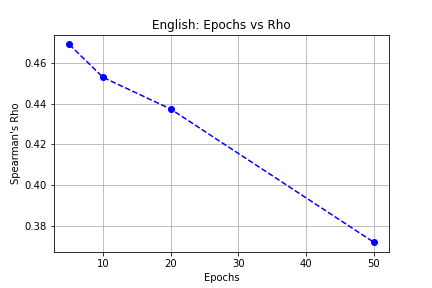
\includegraphics[width = 3in]{sections/figures/top-models/eng_epochs.png}}\quad
  \subcaptionbox{Dimensions}{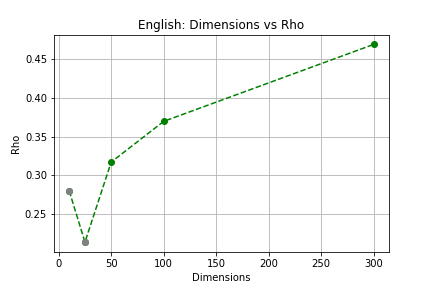
\includegraphics[width = 3in]{sections/figures/top-models/eng_dims.png}}\\
  \subcaptionbox{Frequency Threshold}{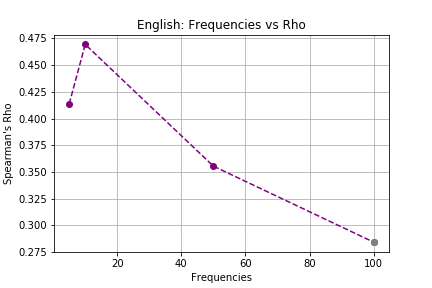
\includegraphics[width = 3in]{sections/figures/top-models/eng_freqs.png}}\quad
  \subcaptionbox{Vocabulary Size}{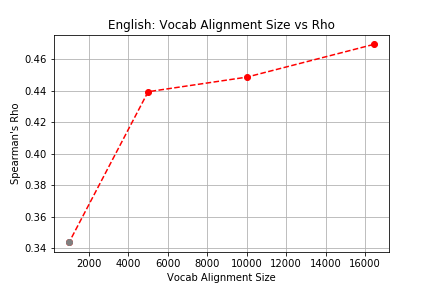
\includegraphics[width = 3in]{sections/figures/top-models/eng_vocabalign.png}}
  \caption{English Top Model Hyperparamater Graphs}
  \label{fig:eng-topmodels}
\end{figure}



\pagebreak

\vspace*{\fill}

\begin{figure}[h]
  \centering
  \subcaptionbox{Epochs}{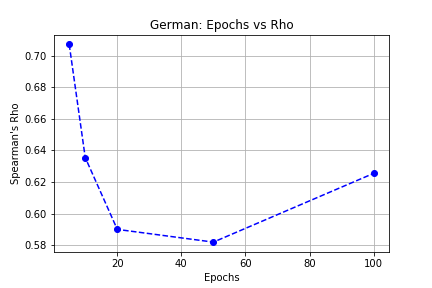
\includegraphics[width = 3in]{sections/figures/top-models/deu_epochs.png}}\quad
  \subcaptionbox{Dimensions}{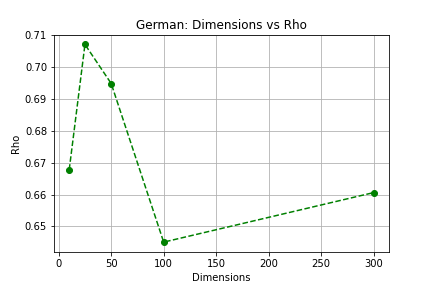
\includegraphics[width = 3in]{sections/figures/top-models/deu_dims.png}}\\
  \subcaptionbox{Frequency Threshold}{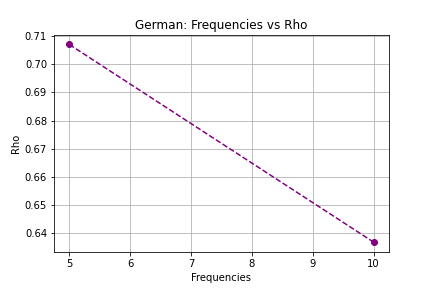
\includegraphics[width = 3in]{sections/figures/top-models/deu_freqs.png}}\quad
  \subcaptionbox{Vocabulary Size}{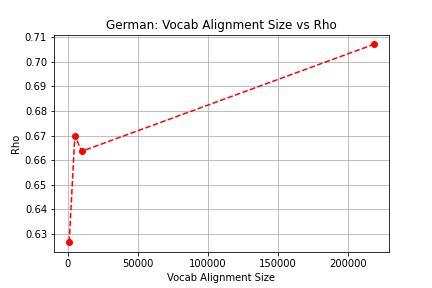
\includegraphics[width = 3in]{sections/figures/top-models/deu_vocabalign.png}}
  \caption{German Top Model Hyperparamater Graphs)}
  \label{fig:deu-topmodels}
\end{figure}

\vspace*{\fill}

\pagebreak

\vspace*{\fill}
 
\begin{figure}[h]
  \centering
  \subcaptionbox{Epochs}{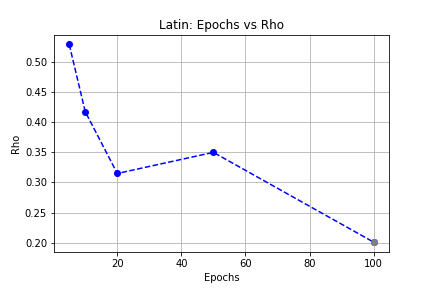
\includegraphics[width = 3in]{sections/figures/top-models/lat_epochs.png}}\quad
  \subcaptionbox{Dimensions}{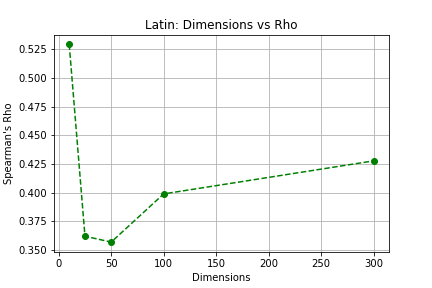
\includegraphics[width = 3in]{sections/figures/top-models/lat_dims.png}}\\
  \subcaptionbox{Frequency Threshold}{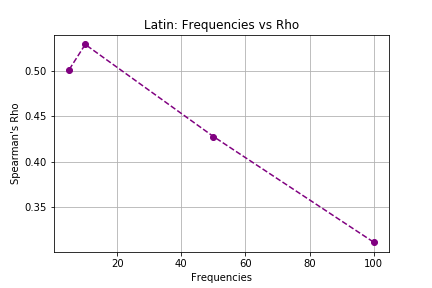
\includegraphics[width = 3in]{sections/figures/top-models/lat_freqs.png}}\quad
  \caption{Latin Top Model Hyperparamater Graphs}
  \label{fig:lat-topmodels}
\end{figure}

\vspace*{\fill}

\pagebreak

\vspace*{\fill}

\begin{figure}[h]
  \centering
  \subcaptionbox{Epochs}{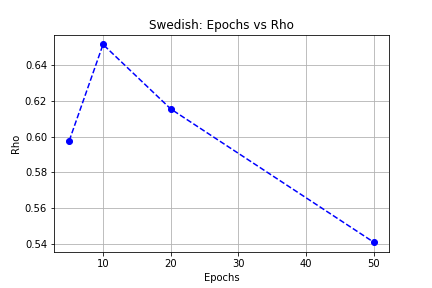
\includegraphics[width = 3in]{sections/figures/top-models/sve_epochs.png}}\quad
  \subcaptionbox{Dimensions}{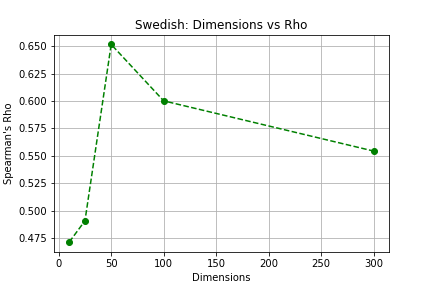
\includegraphics[width = 3in]{sections/figures/top-models/sve_dims.png}}\\
  \subcaptionbox{Frequency Threshold}{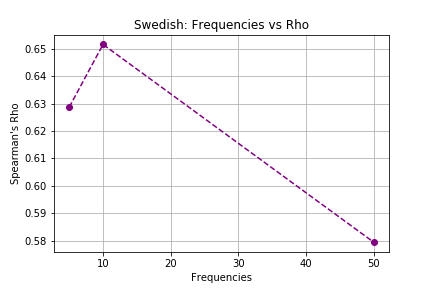
\includegraphics[width = 3in]{sections/figures/top-models/sve_freqs.png}}\quad
  \subcaptionbox{Vocabulary Size}{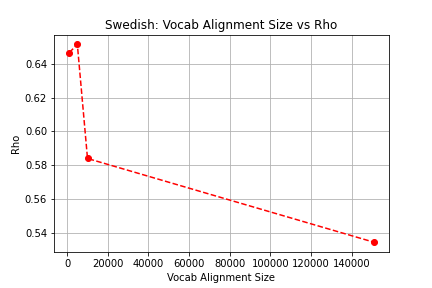
\includegraphics[width = 3in]{sections/figures/top-models/sve_vocabalign.png}}
  \caption{Swedish Top Model Hyperparamater Graphs}
  \label{fig:sve-topmodels}
\end{figure}

\vspace*{\fill}
\section{POS-Tag Target Word Lists and Results}
\label{app-postags}


The following 4 tables are the POS-tagged target word lists for English, German, Latin, and Swedish. The English graded truth labels were already POS-tagged when downloaded from SemEval-2020 Task 1. German, Latin, and Swedish were manually annotated by annotators that have linguistic backgrounds. The tables are ranked by highest change score (Cosine Distance) to lowest. A 0 in cosine distance indicates that the word is a control word and did not undergo any LSC. The number of occurrences for each target word in both corpora are also included. These word lists will be made available to the public.



\begin{table}
\centering
\begin{tabular}{ccccc} 
\toprule
\textbf{ Words } & \textbf{POS } & \textbf{ Cosine Distance} & \textbf{ C$_1$ Freq } & \textbf{ C$_2$ Freq  }  \\ 
\midrule
plane            & nn            & 0.882348                 & 278                & 792                 \\
tip              & vb            & 0.678899                 & 119                & 241                 \\
prop             & nn            & 0.624760                 & 121                & 147                 \\
graft            & nn            & 0.553976                 & 119                & 109                 \\
record           & nn            & 0.427350                 & 420                & 1188                \\
ball             & nn            & 0.409367                 & 440                & 878                 \\
stab             & nn            & 0.400590                 & 92                 & 117                 \\
twist            & nn            & 0.398493                 & 103                & 186                 \\
bit              & nn            & 0.306577                 & 296                & 622                 \\
head             & nn            & 0.295256                 & 3599               & 4127                \\
ounce            & nn            & 0.284899                 & 208                & 189                 \\
rag              & nn            & 0.276515                 & 158                & 208                 \\
player           & nn            & 0.273667                 & 132                & 939                 \\
edge             & nn            & 0.260966                 & 457                & 1072                \\
land             & nn            & 0.223448                 & 2321               & 1624                \\
lass             & nn            & 0.212590                 & 111                & 106                 \\
pin              & vb            & 0.207212                 & 114                & 217                 \\
word             & nn            & 0.179307                 & 4387               & 3166                \\
stroke           & vb            & 0.176231                 & 110                & 227                 \\
circle           & vb            & 0.171087                 & 131                & 245                 \\
part             & nn            & 0.161271                 & 4410               & 3213                \\
donkey           & nn            & 0.160104                 & 118                & 148                 \\
gas              & nn            & 0.159570                 & 155                & 680                 \\
attack           & nn            & 0.143970                 & 454                & 833                 \\
thump            & nn            & 0.142992                 & 89                 & 127                 \\
face             & nn            & 0.137791                 & 3394               & 3932                \\
quilt            & nn            & 0.123145                 & 106                & 189                 \\
lane             & nn            & 0.103720                 & 211                & 289                 \\
multitude        & nn            & 0.100364                 & 214                & 899                 \\
bag              & nn            & 0.100364                 & 475                & 131                 \\
savage           & nn            & 0.096869                 & 504                & 133                 \\
contemplation    & nn            & 0.070839                 & 240                & 111                 \\
tree             & nn            & 0.070839                 & 2322               & 1596                \\
relationship     & nn            & 0.056218                 & 130                & 841                 \\
fiction          & nn            & 0.020723                 & 202                & 326                 \\
risk             & nn            & 0.000000                 & 286                & 643                 \\
chairman         & nn            & 0.000000                 & 147                & 683                 \\
\bottomrule
\end{tabular}
\caption{English Graded Truth Target Words}
\label{tab:eng-truthtargets}
\end{table}



\begin{table}
\centering
\begin{tabular}{ccccc} 
\toprule
\textbf{ Words }   & \textbf{POS } & \textbf{ Cosine Distance } & \textbf{ C$_1$ Freq } & \textbf{ C$_2$ Freq }  \\ 
\midrule
abgebrüht          & adj           & 0.832645           & 64                 & 106                 \\
Ohrwurm            & nn            & 0.832451           & 39                 & 103                 \\
Engpaß             & nn            & 0.819957           & 82                 & 302                 \\
abbauen            & vb            & 0.740115           & 61                 & 1179                \\
ausspannen         & vb            & 0.706690           & 268                & 129                 \\
Eintagsfliege      & nn            & 0.660060           & 59                 & 137                 \\
Knotenpunkt        & nn            & 0.647627           & 360                & 216                 \\
artikulieren       & vb            & 0.615743           & 59                 & 220                 \\
abdecken           & vb            & 0.606884           & 52                 & 366                 \\
Dynamik            & nn            & 0.578845           & 61                 & 681                 \\
Abgesang           & nn            & 0.578548           & 139                & 113                 \\
verbauen           & vb            & 0.578125           & 68                 & 209                 \\
Fuß                & nn            & 0.564633           & 30817              & 3724                \\
Armenhaus          & nn            & 0.519670           & 101                & 127                 \\
zersetzen          & vb            & 0.505880           & 689                & 212                 \\
Rezeption          & nn            & 0.464989           & 101                & 152                 \\
packen             & vb            & 0.462253           & 1806               & 1397                \\
Schmiere           & nn            & 0.437671           & 108                & 122                 \\
Sensation          & nn            & 0.406144           & 170                & 638                 \\
Titel              & nn            & 0.393045           & 3576               & 8637                \\
Mißklang           & nn            & 0.379723           & 54                 & 107                 \\
Manschette         & nn            & 0.355802           & 78                 & 128                 \\
beimischen         & vb            & 0.307359           & 255                & 120                 \\
überspannen        & vb            & 0.252066           & 153                & 194                 \\
vorliegen          & vb            & 0.190266           & 1888               & 1436                \\
Entscheidung       & nn            & 0.141681           & 4030               & 8582                \\
vorweisen          & vb            & 0.126837           & 68                 & 371                 \\
Lyzeum             & nn            & 0.126381           & 107                & 118                 \\
voranstellen       & vb            & 0.124192           & 156                & 194                 \\
Tragfähigkeit      & nn            & 0.114694           & 82                 & 326                 \\
Spielball          & nn            & 0.103290           & 59                 & 176                 \\
Festspiel          & nn            & 0.100364           & 50                 & 708                 \\
Ausnahmegesetz     & nn            & 0.093138           & 59                 & 170                 \\
Gesichtsausdruck   & nn            & 0.077318           & 101                & 157                 \\
Tier               & nn            & 0.073466           & 30574              & 4335                \\
Naturschönheit     & nn            & 0.071561           & 98                 & 130                 \\
vergönnen          & vb            & 0.071197           & 706                & 205                 \\
Frechheit          & nn            & 0.070839           & 362                & 213                 \\
Seminar            & nn            & 0.064486           & 192                & 1975                \\
aufrechterhalten   & vb            & 0.036109           & 40                 & 1171                \\
Unentschlossenheit & nn            & 0.000000           & 76                 & 130                 \\
Ackergerät         & nn            & 0.000000           & 53                 & 106                 \\
Truppenteil        & nn            & 0.000000           & 169                & 630                 \\
Pachtzins          & nn            & 0.000000           & 39                 & 103                 \\
Mulatte            & nn            & 0.000000           & 139                & 116                 \\
Einreichung        & nn            & 0.000000           & 60                 & 141                 \\
weitgreifend       & adj           & 0.000000           & 64                 & 103                 \\
Kubikmeter         & nn            & 0.000000           & 123                & 1903                \\
\bottomrule
\end{tabular}
\caption{German Graded Truth Target Words}
\label{tab:deu-truthtargets}
\end{table}




\begin{table}
\centering
\begin{tabular}{ccccc} 
\toprule
\textbf{ Words } & \textbf{ POS } & \textbf{ Cosine Distance } & \textbf{ C$_1$ Freq } & \textbf{ C$_2$ Freq }  \\ 
\midrule
pontifex         & nn            & 0.905600           & 134                & 1488                \\
imperator        & nn            & 0.846816           & 732                & 10617               \\
beatus           & adj           & 0.816392           & 344                & 2865                \\
sacramentum      & nn            & 0.688040           & 43                 & 1674                \\
titulus          & nn            & 0.619797           & 45                 & 1546                \\
potestas         & nn            & 0.548475           & 913                & 3998                \\
scriptura        & nn            & 0.516652           & 27                 & 1549                \\
licet            & vb            & 0.506818           & 889                & 6043                \\
salus            & nn            & 0.469503           & 671                & 3572                \\
humanitas        & nn            & 0.455671           & 125                & 546                 \\
sanctus          & adj           & 0.425203           & 190                & 10319               \\
virtus           & nn            & 0.397110           & 1643               & 5452                \\
sensus           & nn            & 0.393510           & 431                & 3512                \\
credo            & vb            & 0.370992           & 1660               & 8941                \\
templum          & nn            & 0.370184           & 439                & 3231                \\
nepos            & nn            & 0.364883           & 68                 & 1186                \\
regnum           & nn            & 0.355575           & 700                & 7285                \\
jus              & nn            & 0.350099           & 1209               & 6683                \\
adsumo           & vb            & 0.342616           & 45                 & 338                 \\
dubius           & adj           & 0.337623           & 423                & 2026                \\
civitas          & nn            & 0.322392           & 1693               & 7074                \\
honor            & nn            & 0.290373           & 897                & 4995                \\
dux              & nn            & 0.289054           & 914                & 5128                \\
cohors           & nn            & 0.280830           & 293                & 1032                \\
senatus          & nn            & 0.264773           & 2630               & 2228                \\
sapientia        & nn            & 0.234681           & 306                & 2642                \\
poena            & nn            & 0.230906           & 447                & 3772                \\
nobilitas        & nn            & 0.181606           & 183                & 642                 \\
dolus            & nn            & 0.176682           & 106                & 672                 \\
fidelis          & adj           & 0.170439           & 131                & 2801                \\
acerbus          & adj           & 0.169367           & 149                & 349                 \\
voluntas         & nn            & 0.144737           & 536                & 3214                \\
consul           & nn            & 0.129886           & 3992               & 2513                \\
consilium        & nn            & 0.102932           & 1772               & 4926                \\
oportet          & vb            & 0.102492           & 1278               & 3414                \\
necessarius      & adj           & 0.095190           & 409                & 2978                \\
itero            & vb            & 0.039678           & 32                 & 247                 \\
simplex          & adj           & 0.009540           & 143                & 2141                \\
hostis           & nn            & 0.000000           & 3088               & 6033                \\
ancilla          & nn            & 0.000000           & 96                 & 603                 \\
\bottomrule
\end{tabular}
\caption{Latin Graded Truth Target Words}
\label{tab:lat-truthtargets}
\end{table}



\begin{table}
\centering
\begin{tabular}{ccccc} 
\toprule
\textbf{ Words } & \textbf{ POS } & \textbf{ Cosine Distance } & \textbf{ C$_1$ Freq } & \textbf{ C$_2$ Freq }  \\ 
\midrule
medium           & nn            & 0.603554           & 706                & 517                 \\
krita            & nn            & 0.442764           & 473                & 377                 \\
motiv            & nn            & 0.353028           & 147                & 2719                \\
ledning          & nn            & 0.337868           & 1373               & 13459               \\
granskare        & nn            & 0.319612           & 209                & 89                  \\
uppläggning      & nn            & 0.293040           & 164                & 199                 \\
beredning        & nn            & 0.263710           & 765                & 2095                \\
konduktör        & nn            & 0.247635           & 104                & 1897                \\
bearbeta         & vb            & 0.243557           & 249                & 1645                \\
notis            & nn            & 0.212213           & 241                & 4705                \\
uppfattning      & nn            & 0.195435           & 83                 & 9044                \\
undertrycka      & vb            & 0.166747           & 254                & 1629                \\
färg             & nn            & 0.163421           & 7087               & 15036               \\
blockera         & vb            & 0.159570           & 736                & 235                 \\
antyda           & vb            & 0.143225           & 3103               & 3685                \\
central          & adj           & 0.122427           & 123                & 4012                \\
kemisk           & adj           & 0.100908           & 108                & 3926                \\
aktiv            & adj           & 0.087075           & 121                & 1461                \\
by               & nn            & 0.074686           & 6953               & 15499               \\
gagn             & nn            & 0.071197           & 899                & 3717                \\
annandag         & nn            & 0.070839           & 751                & 2031                \\
bröllop          & nn            & 0.070839           & 255                & 4702                \\
studie           & nn            & 0.070443           & 906                & 3744                \\
förhandling      & nn            & 0.002218           & 95                 & 9122                \\
bedömande        & vb            & 0.000443           & 130                & 1478                \\
kokärt           & nn            & 0.000000           & 167                & 203                 \\
bolagsstämma     & nn            & 0.000000           & 1270               & 12516               \\
uppfostran       & nn            & 0.000000           & 5066               & 3413                \\
uträtta          & vb            & 0.000000           & 2841               & 3746                \\
vaktmästare      & nn            & 0.000000           & 162                & 2693                \\
vegetation       & nn            & 0.000000           & 156                & 313                 \\
\bottomrule
\end{tabular}
\caption{Swedish Graded Truth Target Words}
\label{tab:sve-truthtargets}
\end{table}


% ----------------
% The tables below show the top-performing models based on the smaller target word lists created by sorting the target words by POS-tag. For each table, the first row is the overall top-performing model (entire target word list) which is included for easier comparisons. 











\end{document}


